%% BioMed_Central_Tex_Template_v1.06
%%                                      %
%  bmc_article.tex            ver: 1.06 %
%                                       %

%%IMPORTANT: do not delete the first line of this template
%%It must be present to enable the BMC Submission system to
%%recognise this template!!

%%%%%%%%%%%%%%%%%%%%%%%%%%%%%%%%%%%%%%%%%
%%                                     %%
%%  LaTeX template for BioMed Central  %%
%%     journal article submissions     %%
%%                                     %%
%%          <8 June 2012>              %%
%%                                     %%
%%                                     %%
%%%%%%%%%%%%%%%%%%%%%%%%%%%%%%%%%%%%%%%%%


%%%%%%%%%%%%%%%%%%%%%%%%%%%%%%%%%%%%%%%%%%%%%%%%%%%%%%%%%%%%%%%%%%%%%
%%                                                                 %%
%% For instructions on how to fill out this Tex template           %%
%% document please refer to Readme.html and the instructions for   %%
%% authors page on the biomed central website                      %%
%% http://www.biomedcentral.com/info/authors/                      %%
%%                                                                 %%
%% Please do not use \input{...} to include other tex files.       %%
%% Submit your LaTeX manuscript as one .tex document.              %%
%%                                                                 %%
%% All additional figures and files should be attached             %%
%% separately and not embedded in the \TeX\ document itself.       %%
%%                                                                 %%
%% BioMed Central currently use the MikTex distribution of         %%
%% TeX for Windows) of TeX and LaTeX.  This is available from      %%
%% http://www.miktex.org                                           %%
%%                                                                 %%
%%%%%%%%%%%%%%%%%%%%%%%%%%%%%%%%%%%%%%%%%%%%%%%%%%%%%%%%%%%%%%%%%%%%%

%%% additional documentclass options:
%  [doublespacing]
%  [linenumbers]   - put the line numbers on margins

%%% loading packages, author definitions

%\documentclass[twocolumn]{bmcart}% uncomment this for twocolumn layout and comment line below
\documentclass[doublespacing]{bmcart}

%%% Load packages
\usepackage{amsthm,amsmath}
%\RequirePackage{natbib}
%\RequirePackage[authoryear]{natbib}% uncomment this for author-year bibliography
\RequirePackage{hyperref}
%\usepackage[utf8]{inputenc} %unicode support
\usepackage[applemac]{inputenc} %applemac support if unicode package fails
%\usepackage[latin1]{inputenc} %UNIX support if unicode package fails
\usepackage{subcaption}


%%%%%%%%%%%%%%%%%%%%%%%%%%%%%%%%%%%%%%%%%%%%%%%%%
%%                                             %%
%%  If you wish to display your graphics for   %%
%%  your own use using includegraphic or       %%
%%  includegraphics, then comment out the      %%
%%  following two lines of code.               %%
%%  NB: These line *must* be included when     %%
%%  submitting to BMC.                         %%
%%  All figure files must be submitted as      %%
%%  separate graphics through the BMC          %%
%%  submission process, not included in the    %%
%%  submitted article.                         %%
%%                                             %%
%%%%%%%%%%%%%%%%%%%%%%%%%%%%%%%%%%%%%%%%%%%%%%%%%


\def\includegraphic{}
\def\includegraphics{}
\usepackage{graphicx}


\usepackage{multirow}
\usepackage{url}

\usepackage{xspace}

\newcommand\nd{\textsuperscript{nd}\xspace}
\newcommand\rd{\textsuperscript{rd}\xspace}
\newcommand\nth{\textsuperscript{th}\xspace} %\th is taken already

%%% Put your definitions there:
\startlocaldefs
\newcommand{\pv}{\textit{P. vivax}}
\newcommand{\pf}{\textit{P. falciparum}}
\newcommand{\males}{M15$+$}
\newcommand{\gen}{Gen}
\newcommand{\pq}{PQ}
\graphicspath{{../figures/}}
\endlocaldefs


%%% Begin ...
\begin{document}

%%% Start of article front matter
\begin{frontmatter}

\begin{fmbox}
\dochead{Research}

%%%%%%%%%%%%%%%%%%%%%%%%%%%%%%%%%%%%%%%%%%%%%%
%%                                          %%
%% Enter the title of your article here     %%
%%                                          %%
%%%%%%%%%%%%%%%%%%%%%%%%%%%%%%%%%%%%%%%%%%%%%%

\title{Is a radical cure enough? Assessing a primaquine treatment for adult males in Cambodia to eliminate vivax malaria by 2025}

%%%%%%%%%%%%%%%%%%%%%%%%%%%%%%%%%%%%%%%%%%%%%%
%%                                          %%
%% Enter the authors here                   %%
%%                                          %%
%% Specify information, if available,       %%
%% in the form:                             %%
%%   <key>={<id1>,<id2>}                    %%
%%   <key>=                                 %%
%% Comment or delete the keys which are     %%
%% not used. Repeat \author command as much %%
%% as required.                             %%
%%                                          %%
%%%%%%%%%%%%%%%%%%%%%%%%%%%%%%%%%%%%%%%%%%%%%%

%\author[
%   addressref={aff1},                   % id's of addresses, e.g. {aff1,aff2}
%   corref={aff1},                       % id of corresponding address, if any
%   noteref={n1},                        % id's of article notes, if any
%   email={jane.e.doe@cambridge.co.uk}   % email address
%]{\inits{JE}\fnm{Jane E} \snm{Doe}}
%\author[
%   addressref={aff1,aff2},
%   email={john.RS.Smith@cambridge.co.uk}
%]{\inits{JRS}\fnm{John RS} \snm{Smith}}
\author[
   addressref={bi},
   email={rowan.martin-hughes@burnet.edu.au}
]{\inits{R}\fnm{Rowan} \snm{Martin-Hughes}}
%
\author[
   addressref={bi,melbms,jcu,csiro},                   % id's of addresses, e.g. {aff1,aff2}
   %corref={aff1},                       % id of corresponding address, if any
   %noteref={n1},                        % id's of article notes, if any
   email={r.hickson@UNSWalumni.com}   % email address
]{\inits{RI}\fnm{RI} \snm{Hickson}}
%
\author[
   addressref={menzies},
   email={angela.devine@menzies.edu.au}
]{\inits{A}\fnm{Angela} \snm{Devine}}
%
\author[
   addressref={melbph,doherty},
   email={david.price1@unimelb.edu.au}
]{\inits{DJ}\fnm{David J} \snm{Price}}
\author[
   addressref={menzies},
   email={kamala.ley-thriemer@menzies.edu.au}
]{\inits{K}\fnm{Kamala} \snm{Thriemer}}
%
% from here, excepting senior, authors are alphabetical
\author[
   addressref={bi},
   email={freya.fowkes@burnet.edu.au}
]{\inits{FJI}\fnm{Freya JI} \snm{Fowkes}}
%
\author[
   addressref={melbms,melbph,doherty},
   email={jamesm@unimelb.edu.au}
]{\inits{JM}\fnm{James M} \snm{McCaw}}
%
\author[
   addressref={melbph},
   email={julieas@unimelb.edu.au}
]{\inits{JA}\fnm{Julie A} \snm{Simpson}}
%
\author[
   addressref={bi},
   email={romesh.abeysuriya@burnet.edu.au}
]{\inits{RA}\fnm{Romesh} \snm{Abeysuriya}}
%
\author[
   addressref={bi},
   email={nick.scott@burnet.edu.au }
]{\inits{NS}\fnm{Nick} \snm{Scott}}
%
\author[
   addressref={cnm},
   email={sivsovannaroths@gmail.com}
]{\inits{S}\fnm{Siv} \snm{Sovannaroth}}
%
\author[
   addressref={cnm,moru},
   email={pengby@email.com}
]{\inits{P}\fnm{Pengby} \snm{Ngor}}

%%%%%%%%%%%%%%%%%%%%%%%%%%%%%%%%%%%%%%%%%%%%%%
%%                                          %%
%% Enter the authors' addresses here        %%
%%                                          %%
%% Repeat \address commands as much as      %%
%% required.                                %%
%%                                          %%
%%%%%%%%%%%%%%%%%%%%%%%%%%%%%%%%%%%%%%%%%%%%%%

%\address[id=aff1]{%                           % unique id
%  \orgname{Department of Zoology, Cambridge}, % university, etc
%  %\street{Waterloo Road},                     %
%  %\postcode{}                                % post or zip code
%  \city{London},                              % city
%  \cny{UK}                                    % country
%}
%\address[id=aff2]{%
%  \orgname{Marine Ecology Department, Institute of Marine Sciences Kiel},
%  %\street{D\"{u}sternbrooker Weg 20},
%  %\postcode{24105}
%  \city{Kiel},
%  \cny{Germany}
%}
\address[id=bi]{%
  \orgname{Burnet Institute},
  %\street{},
  %\postcode{24105}
  \city{Melbourne},
  \cny{Australia}
}
\address[id=melbms]{%                           % unique id
  \orgname{School of Mathematics and Statistics, Faculty of Science, University of Melbourne}, % university, etc
  %\street{},                     %
  %\postcode{}                                % post or zip code
  \city{Parkville},                              % city
  \cny{Australia}                                    % country
}
\address[id=jcu]{%                           % unique id
  \orgname{College of Public Health, Medical \& Veterinary Sciences; and Australian Institute of Tropical Health \& Medicine, James Cook University}, % university, etc
  %\street{},                     %
  %\postcode{}                                % post or zip code
  \city{Townsville},                              % city
  \cny{Australia}                                    % country
}
\address[id=csiro]{%                           % unique id
  \orgname{Health \& Biosecurity, CSIRO}, % university, etc
  %\street{},                     %
  %\postcode{}                                % post or zip code
  \city{Townsville},                              % city
  \cny{Australia}                                    % country
}
\address[id=melbph]{%
  \orgname{Centre for Epidemiology and Biostatistics, Melbourne School of Population and Global Health, Faculty of Medicine, Dentistry, and Health Sciences, University of Melbourne}, % university, etc
  %\street{},                     %
  %\postcode{}                                % post or zip code
  \city{Parkville},                              % city
  \cny{Australia}                                    % country
}

\address[id=menzies]{%
  \orgname{Menzies School of Health Research},
  %\street{},
  %\postcode{24105}
  \city{Melbourne},
  \cny{Australia}
}
\address[id=doherty]{%
  \orgname{Doherty Institute},
  %\street{},
  %\postcode{24105}
  \city{Melbourne},
  \cny{Australia}
}
\address[id=cnm]{%
  \orgname{Cambodian National Center for Parasitology, Entomology and Malaria Control},
  %\street{},
  %\postcode{24105}
  \city{Phnom Penh},
  \cny{Cambodia}
}
\address[id=moru]{%
  \orgname{Mahidol-Oxford Tropical Medicine Research Unit, Faculty of Tropical Medicine, Mahidol University},
  %\street{},
  %\postcode{24105}
  \city{Bangkok},
  \cny{Thailand}
}

%%%%%%%%%%%%%%%%%%%%%%%%%%%%%%%%%%%%%%%%%%%%%%
%%                                          %%
%% Enter short notes here                   %%
%%                                          %%
%% Short notes will be after addresses      %%
%% on first page.                           %%
%%                                          %%
%%%%%%%%%%%%%%%%%%%%%%%%%%%%%%%%%%%%%%%%%%%%%%

% \begin{artnotes}
% %\note{Sample of title note}     % note to the article
% %\note[id=n1]{Equal contributor} % note, connected to author
% \end{artnotes}

\end{fmbox}% comment this for two column layout

\clearpage 
%%%%%%%%%%%%%%%%%%%%%%%%%%%%%%%%%%%%%%%%%%%%%%
%%                                          %%
%% The Abstract begins here                 %%
%%                                          %%
%% Please refer to the Instructions for     %%
%% authors on http://www.biomedcentral.com  %%
%% and include the section headings         %%
%% accordingly for your article type.       %%
%%                                          %%
%%%%%%%%%%%%%%%%%%%%%%%%%%%%%%%%%%%%%%%%%%%%%%

\begin{abstractbox}
% Instructions from: https://malariajournal.biomedcentral.com/submission-guidelines/preparing-your-manuscript/research-article
%Abstract
%The Abstract should not exceed 350 words. Please minimize the use of abbreviations and do not cite references in the abstract. Reports of randomized controlled trials should follow the CONSORT extension for abstracts. The abstract must include the following separate sections:
%
%Background: the context and purpose of the study
%Methods: how the study was performed and statistical tests used
%Results: the main findings
%Conclusions: brief summary and potential implications
%Trial registration: If your article reports the results of a health care intervention on human participants, it must be registered in an appropriate registry and the registration number and date of registration should be in stated in this section. If it was not registered prospectively (before enrollment of the first participant), you should include the words 'retrospectively registered'. See our editorial policies for more information on trial registration

\begin{abstract} % abstract

\parttitle{Background} %the context and purpose of the study
Elimination targets for \textit{Plasmodium vivax} are approaching, with the Cambodian target 2025. Quantitative tools can assess if proposed strategies are likely to be sufficient to meet those targets.

\parttitle{Methods} %how the study was performed and statistical tests used
We calibrated the Optima Malaria transmission model to reported case data from 2011--2018 for six provinces with different transmission levels. The model had two human populations: males aged 15 years and older, and everyone else. We assessed the addition to the 2018 status quo of a new low dose primaquine intervention (0.25 mg/kg daily x 14 days) for diagnosed \pv~infections where males aged 15 years and older were prescribed primaquine after testing glucose-6-phosphate-dehydrognase normal. Results were evaluated over stochastic iterations of the calibrated compartmental model, incorporating best and worst case interpretations of the available case data given uncertainty over underlying \pv~incidence in 2020.

\parttitle{Results} %the main findings
%The proportion of model trajectories in which \pv~elimination was projected with the addition of the radical cure primaquine intervention was highly dependent on the underlying inputs for \pv~incidence. 
Under 2018 status quo conditions in the absence of a primaquine radical cure, we found that \pv~elimination would be unlikely to be achieved by 2040 in any province. Elimination by 2025 was not projected in any province even with best case assumptions for primaquine intervention coverage, G6PD-based eligibility, and primaquine efficacy, but we estimated that the addition of the primaquine intervention could reduce \pv~transmission by 67\%-83\% by 2025. We found that sustained application of the primaquine intervention was likely to result in elimination by 2040 in all six provinces with best case estimated baseline incidence, and in the two lowest incidence provinces with worst case baseline incidence. 

\parttitle{Conclusions}
Without additional novel interventions, the primaquine radical cure (0.25 mg/kg daily x 14 days targeting adult males with diagnosed \pv~infections) is not projected to result in elimination from any province by the 2025 target even under the most optimistic interpretation of the available case data. However, the implementation of a primaquine intervention in Cambodia is likely to have a substantial impact on transmission of \pv~and may make elimination feasible over the longer term. 

\end{abstract}

%%%%%%%%%%%%%%%%%%%%%%%%%%%%%%%%%%%%%%%%%%%%%%
%%                                          %%
%% The keywords begin here                  %%
%%                                          %%
%% Put each keyword in separate \kwd{}.     %%
%%                                          %%
%%%%%%%%%%%%%%%%%%%%%%%%%%%%%%%%%%%%%%%%%%%%%%

\begin{keyword}
\kwd{Malaria}
\kwd{\textit{Plasmodium vivax}}
\kwd{Transmission}
\kwd{Primaquine}
\kwd{Radical cure}
\kwd{Mathematical model}
\end{keyword}

% MSC classifications codes, if any
%\begin{keyword}[class=AMS]
%\kwd[Primary ]{}
%\kwd{}
%\kwd[; secondary ]{}
%\end{keyword}

\end{abstractbox}
%
%\end{fmbox}% uncomment this for twcolumn layout

\end{frontmatter}
\captionsetup{width=.9\linewidth}

%%%%%%%%%%%%%%%%%%%%%%%%%%%%%%%%%%%%%%%%%%%%%%
%%                                          %%
%% The Main Body begins here                %%
%%                                          %%
%% Please refer to the instructions for     %%
%% authors on:                              %%
%% http://www.biomedcentral.com/info/authors%%
%% and include the section headings         %%
%% accordingly for your article type.       %%
%%                                          %%
%% See the Results and Discussion section   %%
%% for details on how to create sub-sections%%
%%                                          %%
%% use \cite{...} to cite references        %%
%%  \cite{koon} and                         %%
%%  \cite{oreg,khar,zvai,xjon,schn,pond}    %%
%%  \nocite{smith,marg,hunn,advi,koha,mouse}%%
%%                                          %%
%%%%%%%%%%%%%%%%%%%%%%%%%%%%%%%%%%%%%%%%%%%%%%

%%%%%%%%%%%%%%%%%%%%%%%%% start of article main body
% <put your article body there>

%%%%%%%%%%%%%%%%
%% Background %%
%%
%Instructions for authors from: https://malariajournal.biomedcentral.com/submission-guidelines/preparing-your-manuscript/research-article
%Background
%The Background section should explain the background to the study, its aims, a summary of the existing literature and why this study was necessary or its contribution to the field.
\section*{Background} 

\textit{Plasmodium vivax} is the cause of a significant burden of malaria globally, with an estimated 14.3 million cases in 2017~\cite{Battle2019}. Cambodia has reported no malaria deaths since 2018 \cite{WHOmalaria2021}, but with the rise of artemisinin-resistant \textit{Plasmodium falciparum} in Cambodia, the relative burden of \pv~has increased due to increased focus on eliminating \pf. Vivax malaria is now responsible for 30--90\% of cases across the provinces in Cambodia~\cite{WHOmalaria2021, lek2020tools, Sandfort2020}. The standard treatment for blood stage malaria infection in Cambodia is chloroquine (CQ), but this treatment does not clear the dormant liver parasites, called hypnozoites. The hypnozoite stage of \pv~results in relapses~\cite{Douglas2013, Commons2019}, and is a key difference between \pf~and \pv. Additionally targeting the hypnozoite reservoir with a radical cure is considered a key element of control since an estimated 79\% of \pv~episodes are due to relapse \cite{commons2020estimating, thriemer2021towards}.   

The only widely available drug for radical cure is primaquine (PQ). The World Health Organization (WHO) recommendation is to test for G6PD deficiency before administration of \pq~where possible, in order to avoid the primaquine-induced haemolysis that can result in those with this enzymopathy~\cite{WHO2015malaria}. G6PD deficiency is measured by enzymatic activity, and a value of less than 30\% is considered severe deficiency. Since G6PD deficiency is x-linked, females may be homozygous or heterozygous. The latter is more challenging to detect as some will have intermediate activity ($>$30-70\%) and still be at risk of severe haemolysis~\cite{Chu2017}. 

The WHO defines malaria elimination as ``Interruption of local transmission (reduction to zero incidence of indigenous cases) of a specified malaria parasite in a defined geographical area as a result of deliberate activities." \cite{who_2019_definitions}.The elimination target for \pv~in Cambodia is 2025~\cite{Cambodia}. \pq~has been recommended as a radical cure for \pv~in the National Treatment Guidelines for Malaria since 2012~\cite{nattreat_guide2014}, but practical adoption of \pq~as a first-line treatment has been hampered by historical complications resulting from use of \pq~as part of mass drug administration in Cambodia~\cite{kitchakarn2017implementation}. In November 2019, Cambodia began trialling the use of a 14-day low-dose \pq~intervention for adult males with a diagnosed \pv~infection testing G6PD normal with qualitative G6PD rapid diagnostic tests (RDTs) in two health centres in Pursat province~\cite{pursat_protocol2019}, and has since rolled this out as part of the national programme (Table \ref{tab:trialtimeline}). Ongoing policy changes to safely implement the effective radical cure for \pv~in Cambodia are an important part of the regional strategy malaria elimination strategy~\cite{ruwanpura2021further}. 

\begin{table}[]
    \centering
    \begin{tabular}{l l l}
    \hline
    Type of test/treatment & Timeline & Geographical area \\
    \hline
    G6PD qualitative test (CareStart)+ & Sep. 2019 -- training & 4 pilot provinces \\
    PQ14 for males 20kg  & Oct 2019 -- distribution of tests & \\
    & Nov. 2019 -- started trial & \\
    & Dec. 2020 -- ended trial & \\
    \hline
    G6PD quantitative test (SD Biosensor)+  & Oct. to Nov. 2020 -- training & Whole country \\
    PQ14 for all 20kg+ & Jan. 2021 -- distribution of tests & \\
    & Feb. 2021 -- started implementation & \\
    \hline
    
    \end{tabular}
    \caption{Trial and implementation timeline of the primaquine intervention in Cambodia}
    \label{tab:trialtimeline}
\end{table}



We used transmission modelling to inform the planning process of the Cambodia National Center for Parasitology, Entomology and Malaria Control (CNM) in early 2020 to determine if this intervention would be likely to be sufficient to eliminate \pv~by the 2025 target. 



%Methods
%The methods section should include:
%
%the aim, design and setting of the study
%the characteristics of participants or description of materials
%a clear description of all processes, interventions and comparisons. Generic drug names should generally be used. When proprietary brands are used in research, include the brand names in parentheses
%the type of statistical analysis used, including a power calculation if appropriate
\section*{Methods} \label{sec:methods} %Subsections are currently modelled on Scott et al. 2017

\subsection*{Data sources and synthesis} 
Demographic data, including mortality, were obtained from the National Institute of Statistics in Cambodia~\cite{NIS_Cambodia}. The demographic data was from the 2008, 2013, and 2019 census~\cite{NIS_Cambodia}, including estimated population size, known age and gender breakdown, and life expectancy.

Malaria case data were obtained from the CNM. The raw data included total number of tests, and numbers of positive tests by parasite species, test type (microscopy or Deepstick, a rapid diagnostic test), province, and week of test. Additionally, population stratification for estimated \pv~incidence was provided as a proportion of cases by age and sex, from January 2015--November 2019. Subsequently, the raw data for each province was pro rated to achieve the correct proportion of cases for \males, since they are the target sub-population for the \pq~intervention.

%The aggregated data used for model calibration are provided in Additional file~\ref{supp}.

\subsection*{Epidemic model}

The dynamic transmission model of \pv~is based on that by Scott~\etal~\cite{scott2017} used to model \pf. It is a compartmental model that accounts for transmission between humans and mosquitoes, with the disease progression in the model depicted in Fig~\ref{fig:model_flow} including adjustments to account for \pv~further detailed in the Supplemental appendix. The model includes compartments for humans encapsulating disease states: ``Susceptible''; ``Latent'' infected with \pv~in the liver only (hypnozoites and/or active liver stage); ``Active'' infected with active blood stage infection able to infect mosquitoes (gametocytes present), further divided into exposed (during incubation prior to symptoms), uncomplicated or clinical, severe (rare in \pv~infections but present in low numbers in case data for Cambodia), and asymptomatic (including chronic malaria and natural resistance from prior exposure); or ``Recovered/immune'' (with no hypnozoites). Each model compartment without active malarial symptoms (susceptible, latent, and asymptomatic) is stratified to include the possibility of non-malarial fevers, screening, and the potential for false-positive treatment as a result. The recovered and immune compartment is important for capturing \pv~dynamics given our current understanding of the importance of immunity in reducing transmission or symptomatic infections~\cite{mueller2013natural}. The human population is stratified into males 15 years and older (\males) and everyone else (\gen), to enable the \pq~intervention proposed in Cambodia to be captured by the model. To capture the possibility of elimination, the model was run with stochastic transitions between compartments, based on the probability of each individual transitioning during each 5 day timestep.

\begin{figure}[h!]
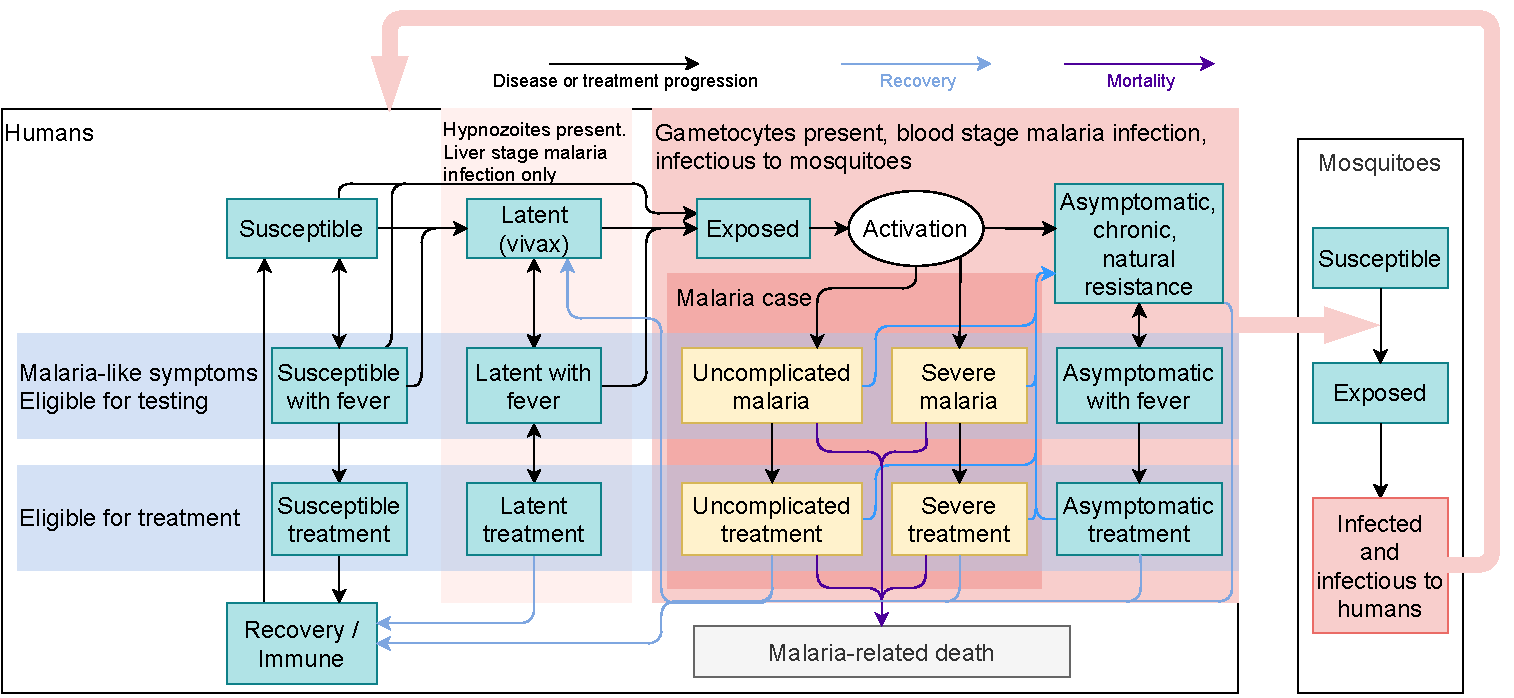
\includegraphics[width=.95\linewidth]{Optima_Malaria_model_diagram.pdf}\caption{\csentence{Optima Malaria model diagram}}\label{fig:model_flow}
\end{figure}


\subsection*{Model calibration} \label{sec:calibration} % and validation 

Data on annual incidence (2011--2018), testing numbers, and demographics were used to calibrate the model for each population stratification (i.e. males 15 years and over, and everyone else) and province. 

The population size was modelled in each province by group, including transitions from \gen~to \males~to represent aging of male children. The population model (births, deaths, and transitions) was initialized to match reported population sizes in 2011 and calibrated to fit the demographics of each province to 2019, based on the National Institute of Statistics in Cambodia data~\cite{NIS_Cambodia}.

The case data was divided into 6 clusters by positive \pv~test results in 2018, as shown in Table~\ref{tab:clusters}, and a province was chosen at random from each cluster to generate a representative selection of \pv~incidence levels across provinces. Pursat was deliberately chosen in keeping with the first \pq~trial location. Provinces where the borders had changed during 2011--2018 were excluded from being chosen to ensure consistency of reported data. In addition to Pursat, the other five provinces selected for our analyses were Mondulkiri, Kampong Chhnang, Battambang, Pailin, and Takeo. 

%{\tiny
%\begin{table}
%\begin{center}
%\begin{tabular}{c c c c c c}
%\hline
%3000 -- 5000 & 1000 -- 3000 & 500 -- 1000 & 120--500 & 0 -- 120 \\ 
%\hline
%Preah Vihear & Kratie & Siem Reap & Preah Sihanouk & Prey Veng \\
%Kampong Speu & Ratanakiri & \emph{Battambang} & \emph{Takeo} & Kandal \\
%\emph{Mondulkiri} & \emph{Kampong Chhnang} & Kampong Thom & Koh Kong & \emph{Pailin} \\
%Stung Treng & Kampong Cham & Kampot & Phnom Penh & Banteay Meanchey \\
%& Oddar Meanchey & & & Kep \\
%& & & & Svay Rieng \\
%\hline
%\end{tabular}
%\end{center}
%\caption{Clustering of provinces by pro rated reported 2018 \pv~case numbers.\\
%\emph{Pursat} selected as the sixth province with $5000+$ pro rata reported cases}\label{tab:clusters}
%\end{table}
%}

{\tiny
\begin{table}
\begin{center}
\begin{tabular}{c c c c}
\hline
Cluster & Province & Pro rata 2018 \pv~cases & 2018 Population \\
\hline
5000+ & \emph{Pursat} & 9,245 & 411,759\\
\hline
\multirow{4}{*}{3000--5000}& Preah Vihear & 4,092 & 251,352\\
& Kampong Speu & 3,569 & 872,219\\
& \emph{Mondulkiri} & 3,464 & 88,649\\
& Stung Treng & 3,204 & 159,565\\
\hline
\multirow{5}{*}{1000--3000}& Kratie & 2,518 & 372,825\\
& Ratanakiri & 2,214 & 204,027\\
& \emph{Kampong Chhnang} & 1,956 & 525,932\\
& Kampong Cham & 1,774 & 895,763\\
& Oddar Meanchey & 1,376 & 261,252\\
\hline
\multirow{4}{*}{500--1000}& Siem Reap & 853 & 1,006,512\\
& \emph{Battambang} & 783 & 987,400\\
& Kampong Thom & 765 & 677,260\\
& Kampot & 500 & 592,845\\
\hline
\multirow{4}{*}{120--500}& Preah Sihanouk & 353 & 302,887\\
& \emph{Takeo} & 281 & 899,485\\
& Koh Kong & 190 & 123,618\\
& Phnom Penh & 143 & 2,129,371\\
\hline
\multirow{6}{*}{0--120}& Prey Veng & 115 & 1,057,428\\
& Kandal & 110 & 1,195,547\\
& \emph{Pailin} & 101 & 71,600\\
& Banteay Meanchey & 76 & 859,545\\
& Kep & 27 & 41,798\\
& Svay Rieng & 22 & 524,554\\
\hline

\end{tabular}
\end{center}
\caption{Clustering of provinces by pro rated reported 2018 \pv~case numbers, with modelled provinces highlighted.\label{tab:clusters}\\
%\emph{Pursat} selected as the sixth province with $5000+$ pro rata reported cases}\label{tab:clusters}
}
\end{table}
}



The following key model parameters with substantial uncertainty were calibrated to fit the incidence and test data using parameters based on deterministic modelling of transmission (e.g. with fractional transfers of a proportion of the population in a model compartment, rather than stochastic transfers of individuals between model compartments): \begin{itemize}
\item the relative susceptibility of the population group to malaria infection given prevailing local conditions (unitless, with \males~being 7 to 11-times more susceptible than \gen); 
\item the rate of developing malaria-like symptoms for each person in a given year for reasons other than malaria (ranging from less than 0.01 to 0.15 in \males~by province, with higher values historically); 
\item the daily rate of testing for people with non-severe malaria-like symptoms such as fever (0.03, representing a 26\% probability of testing within the median 10 day symptomatic duration); 
\item the daily rate of testing for people with severe malaria-like symptoms (0.15, representing an 80\% probability of testing within the median 10 day symptomatic duration); and 
\item the average duration of the latent period (i.e. until hypnozoite reactivation) (76 days, capturing a lower limit of approximately three weeks as reported for Cambodia \cite{white2011determinants}~as well as the potential for some much longer individual durations);
\end{itemize} See the Supplementary appendix for additional parameterization and calibration details. To allow for changes in the surveillance system in Cambodia, and changes in the other interventions through time, we calibrated to both a ``high'' and a ``low'' baseline incidence scenario. The ``high'' scenario is for the true incidence to be consistent with the reported 2018 \pv~incidence data, with a projection of increasing incidence based on the historically lower reported case data relative to 2018, and the ``low'' scenario is for the true incidence to be consistent with the historical values prior to 2018 and following the decreasing trend within those values. The true values for incidence very likely lie within this range, and our approach enables us to capture both the best and worst case baseline scenario for elimination. Uncertainty bounds on the model results were generated by sampling within $\pm10\%$ of the calibrated parameter values and running with stochastic transmission of malaria over repeated iterations, with rejection and replacement of any samples outside of $\pm50\%$ of the calibrated 2018 value of malaria cases due to the wide uncertainty on those values in either scenario. Based on qualitatively identical model runs from two different random seeds with 100 iterations with no more than $\pm10\%$ in the proportion of scenarios reaching elimination by 2040 in each province, a final independently seeded run was conducted with 300 iterations. Uncertainty bounds represent 95\% of the subsequent range.

\subsection*{Primaquine intervention}
In order to directly estimate the impact of low-dose \pq~(dose of 0.25 mg/kg daily x 14 days, although this is defined in the Cambodian national treatment guidelines as standard-dose relative to the lower dose used as preventive therapy for \pf~\cite{nattreat_guide2014}) use in \males~with diagnosed \pv~infections, this is the only programmatic response explicitly considered in the model. The effect of all other interventions that were in use during and prior to 2018 are considered to be captured by the model calibration, and include testing and treatment, the distribution of long-lasting insecticidal nets, malaria education to households, early diagnosis and treatment programs through case finding, case management and reporting, and complementary activities supported by civil society organizations in support of malaria elimination \cite{cmep_q2_2021}. More than 75\% of malaria cases reported between January 2015 and November 2019 in CNM malaria case data were in the \males population, so best case coverage of the \pq~intervention has the potential to reach a large portion of malaria cases.

The \pq~programmatic response is considered to have four key parameters: start date of October 2020 ($D$), coverage ($c$), eligibility for \pq~based on the proportion of males with diagnosed \pv~infections and no G6PD deficiency incorporating RDT sensitivity ($G$), and the effectiveness of \pq~in terms of hypnozoite removal ($E$: a combination of efficacy and adherence). The baseline scenario has no \pq, and a default proportion of $0.75$ of the population not clearing hypnozoites on successful treatment completion~\cite{commons2020estimating}. Therefore, from the start date, each member of the population successfully completing treatment has a probability of $0.75(1-c)(1-G)(1-E)$ of not clearing hypnozoites, capturing attainable coverage, G6PD eligibility, and effectiveness of \pq~respectively.  To determine if elimination of \pv~is possible by 2025, we consider the implementation of three scenarios from October 2020 until December 31 2040.
\begin{description}
\item [2018 status quo] is the baseline with no practical application of a radical cure and a continuation of the most recently reported and calibrated interventions targeting the elimination of \pf.

\item [Best case primaquine males 15+] includes the best case for each parameter estimated to be achievable with 90\% coverage of testing, 90\% eligibility based on G6PD normal results (it has been estimated that prevalence of G6PD deficiency among \males~ranges from 5\% to 15\% in different regions of Cambodia \cite{khim2013g6pd, kim2011performance}), and 88\% efficacy in clearing hypnozoites in those who complete treatment~\cite{commons2020estimating}. This is beyond what was achieved through pilot implementation of G6PD RDTs in 4 provinces, where 45\% of adult males with diagnosed \pv~and mixed infections were tested for G6PD deficiency, with 76\% of those tested being G6PD normal, and 78\% of those completing the 14-day treatment~\cite{brief_g6pdtests_2020}. Although opportunities to increase coverage, improve testing, and increase adherence were identified from this pilot, if \pv~is still present in 2025 in the model results for this best case scenario, \pq~in \males~alone will not be sufficient for elimination.

\item [Perfect radical cure] is a beyond best case scenario in which a perfect (100\% success rate) radical cure is available as part of treatment to 100\% of all diagnosed \pv~cases, with no eligibility constraints based on gender, age, weight, or G6PD deficiency. This scenario captures not just the implementation of the radical cure since February 2021 (Table \ref{tab:trialtimeline}) but any future expansion of eligibility or treatment effectiveness. 
\end{description}

\subsection*{Evaluation of primaquine impact}
Indigenous cases in keeping with the WHO definition of malaria elimination \cite{who_2019_definitions} are captured in the model as new malaria cases (whether symptomatic or asymptomatic) occurring in the susceptible population, excluding relapse cases in people with existing latent \pv~infections. We also evaluate the projected number of diagnosed \pv~cases, and the total burden of people with \pv~parasites present including latent infections, to evaluate how these change over time within each scenario.

As we conducted stochastic modelling with 300 runs, we can analyse the proportion of runs in which elimination is projected to occur under each scenario in each province with each calibration.

%Results
%This should include the findings of the study including, if appropriate, results of statistical analysis which must be included either in the text or as tables and figures.
\section*{Results}

\subsection*{Model calibration}
For each of the 6 provinces, calibrations such as that shown in Fig~\ref{fig:calibration_Pursat} for Pursat were conducted. The left column (a) represents the ``males 15 years and older'' (\males) population group, and the right column (b) the ``everyone else'' (\gen) group. The solid red line represents the ``worst case'' baseline incidence calibration, where the model is calibrated deterministically to the higher data values and increasing trend after 2018. The solid blue line represents the ``best case'', where the model is calibrated to the lower values and has a decreasing trend. Faint lines show each individual sampled model iteration run as a baseline for each intervention scenario. The remaining province calibrations are shown in Figs~\ref{fig:calibration_Mondulkiri}--\ref{fig:calibration_Pailin}.

\begin{figure}[h!]
\centering
\subcaptionbox{M 15+, low.\label{M 15+_low}}{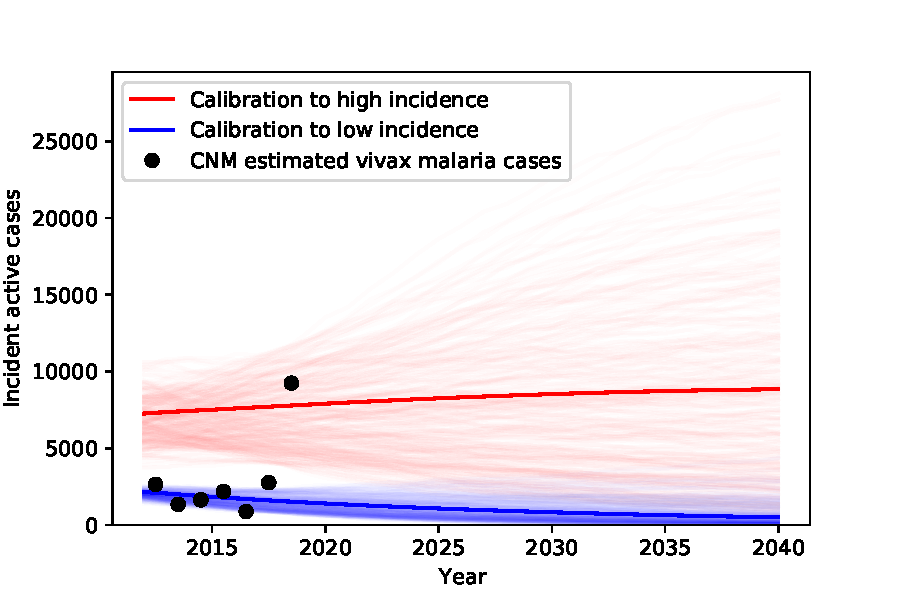
\includegraphics[width=.45\linewidth]{calibration_Pursat_active_cases_M 15+.pdf}} 
\subcaptionbox{Gen, low.\label{Gen_low}}{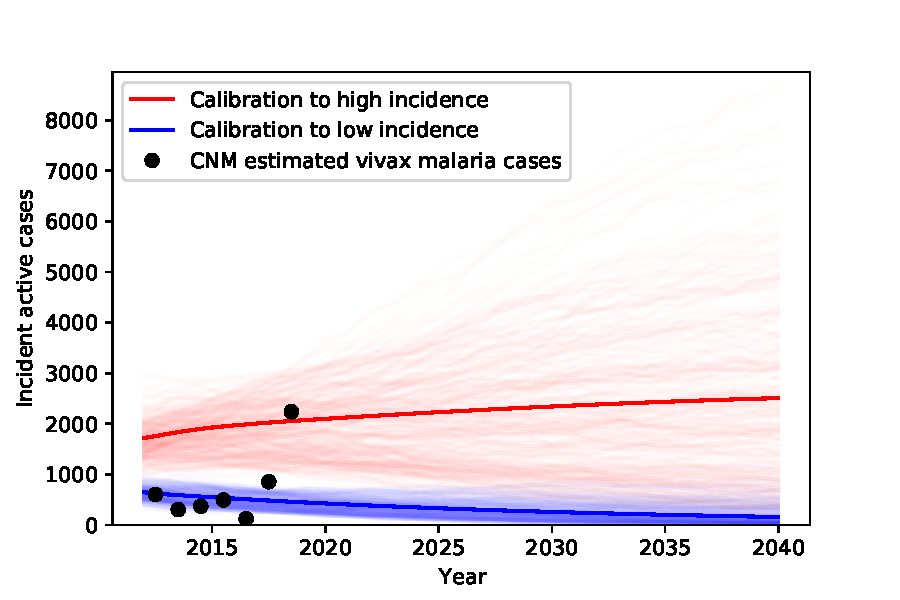
\includegraphics[width=.45\linewidth]{calibration_Pursat_active_cases_Gen.pdf}} 
\caption{\csentence{Calibration to reported \pv~cases in Pursat.} Faint lines represent sampled model trajectories for each of the low and high incidence calibrations.}\label{fig:calibration_Pursat}
\end{figure}

\subsection*{Primaquine impact on burden of disease in Cambodia} \label{sec:impact}

The impact of each radical cure scenario from October 2020, is shown in Fig~\ref{fig:pq_Pursat} for Pursat. The left column (a, c) represents the median projected number of new indigenous cases of \pv~in Pursat from 300 iterations of each scenario, while the right column (b, d) represents the median projected number of total \pv~cases including relapse in Pursat from 300 iterations of each scenario. The top row (a, b) represents the high incidence calibration, while the bottom row (c, d) represents the low incidence calibration. The projected impact of the \pv~radical cure scenarios for the remaining provinces are shown in Figs~\ref{fig:pq_Mondulkiri}--\ref{fig:pq_Pailin}.


\begin{table}
\scriptsize
\begin{center}
%\begin{tabular}{|r | c | c c | c c | c c |}
%\resizebox{\textwidth}{!}{
\begin{tabular}{p{0.23\textwidth}p{0.15\textwidth}p{0.15\textwidth}p{0.15\textwidth}p{0.15\textwidth}}
\hline
Province  & 2019 estimated indigenous cases&2025 projected indigenous cases without radical cure&2025 projected indigenous cases with best case \pq&2025 projected indigenous cases with perfect radical cure \\
\hline
Pursat high & 2,431 (1,462, 3,739)&2,524 (1,149, 4,661)&713 (264, 1,515)&555 (201, 1,250) \\
Pursat low & 440 (278, 681)&292 (137, 639)&81 (28, 264)&59 (16, 234) \\
Mondulkiri high & 777 (516, 1,107)&797 (403, 1,373)&211 (68, 723)&186 (48, 641) \\
Mondulkiri low & 215 (135, 327)&145 (67, 290)&38 (9, 124)&32 (7, 115) \\
Kampong Chhnang high & 360 (244, 574)&395 (205, 879)&117 (47, 268)&89 (31, 236) \\
Kampong Chhnang low & 62 (35, 100)&38 (14, 92)&11 (3, 30)&8 (1, 25) \\
Battambang high & 1,030 (669, 1,607)&1,060 (502, 2,176)&269 (83, 856)&217 (57, 775) \\
Battambang low & 150 (90, 241)&87 (38, 212)&24 (5, 95)&18 (3, 90) \\
Takeo high & 176 (112, 282)&183 (85, 426)&52 (18, 129)&39 (11, 103) \\
Takeo low & 30 (17, 51)&20 (6, 48)&5 (0, 17)&5 (0, 14) \\
Pailin high & 283 (178, 421)&322 (141, 618)&92 (33, 212)&67 (22, 167) \\
Pailin low & 39 (21, 63)&28 (7, 67)&8 (0, 20)&5 (0, 17) \\
\hline
\end{tabular}
%}
\caption{Projected annual \pv~case numbers by province in 2019 baseline and in 2025 under each radical cure scenario. Median of 300 model trajectories (10\nth percentile, 90\nth percentile) as of the respective year}\label{tab:radcure_numbers}
\end{center}
\end{table}

\begin{table}
\scriptsize
\begin{center}
%\begin{tabular}{|r | c | c c | c c | c c |}
%\resizebox{\textwidth}{!}{
\begin{tabular}{p{0.23\textwidth}p{0.2\textwidth}p{0.2\textwidth}p{0.2\textwidth}}
\hline
Province  &2025 projected indigenous cases without radical cure&2025 projected indigenous cases with best case \pq&2025 projected indigenous cases with perfect radical cure \\
\hline
Pursat high & -3\% (-26\%, 25\%)&70\% (53\%, 84\%)&77\% (60\%, 89\%) \\
Pursat low & 32\% (2\%, 53\%)&82\% (51\%, 92\%)&86\% (56\%, 95\%) \\
Mondulkiri high & -3\% (-29\%, 24\%)&73\% (23\%, 88\%)&76\% (31\%, 92\%) \\
Mondulkiri low & 31\% (4\%, 57\%)&83\% (54\%, 94\%)&86\% (58\%, 96\%) \\
Kampong Chhnang high & -9\% (-60\%, 28\%)&68\% (42\%, 85\%)&74\% (51\%, 90\%) \\
Kampong Chhnang low & 36\% (-7\%, 72\%)&82\% (58\%, 95\%)&87\% (66\%, 99\%) \\
Battambang high & -1\% (-37\%, 27\%)&75\% (30\%, 90\%)&80\% (37\%, 92\%) \\
Battambang low & 37\% (3\%, 64\%)&84\% (53\%, 95\%)&88\% (55\%, 97\%) \\
Takeo high & -7\% (-57\%, 35\%)&71\% (45\%, 87\%)&77\% (56\%, 92\%) \\
Takeo low & 30\% (-35\%, 74\%)&83\% (51\%, 100\%)&86\% (56\%, 100\%) \\
Pailin high & -14\% (-57\%, 27\%)&67\% (44\%, 85\%)&75\% (52\%, 91\%) \\
Pailin low & 23\% (-40\%, 73\%)&80\% (57\%, 100\%)&86\% (63\%, 100\%) \\
\hline
\end{tabular}
%}
\caption{Projected percentage reduction in \pv~case numbers by province by 2025 relative to 2019 under each radical cure scenario, relative to status quo for the same underling parameter sample. Median of 300 sampled model trajectories (10\nth percentile, 90\nth percentile) as of 2025.}\label{tab:radcure_percentage}
\end{center}
\end{table}



\begin{figure}[h!]
\centering
\subcaptionbox{Total, high.\label{Pursat_high_indigenous_cases_Total}}{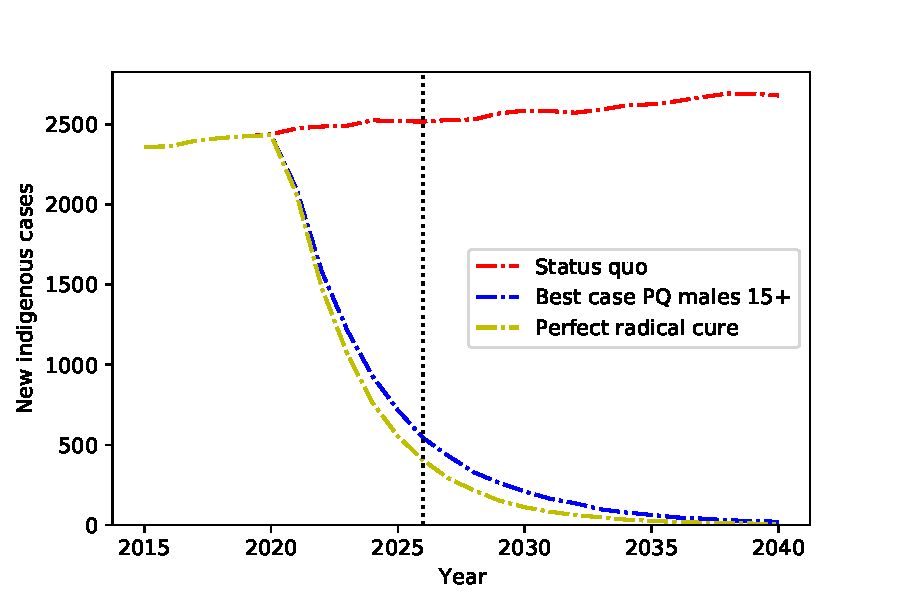
\includegraphics[width=.45\linewidth]{Pursat_high_indigenous_cases_Total.pdf}} 
\subcaptionbox{Total, high.\label{Pursat_high_active_cases_Total}}{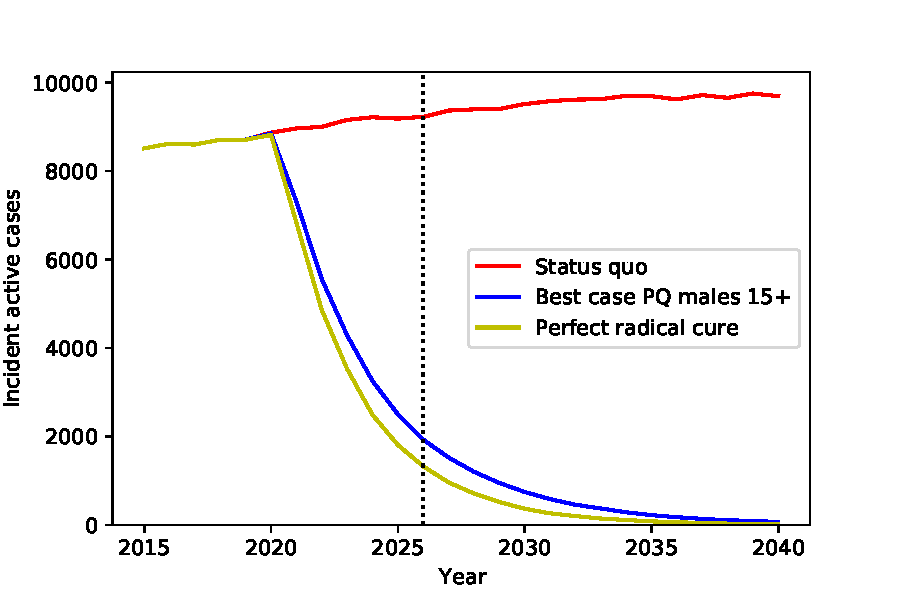
\includegraphics[width=.45\linewidth]{Pursat_high_active_cases_Total.pdf}} 
\subcaptionbox{Total, low.\label{Pursat_low_indigenous_cases_Total}}{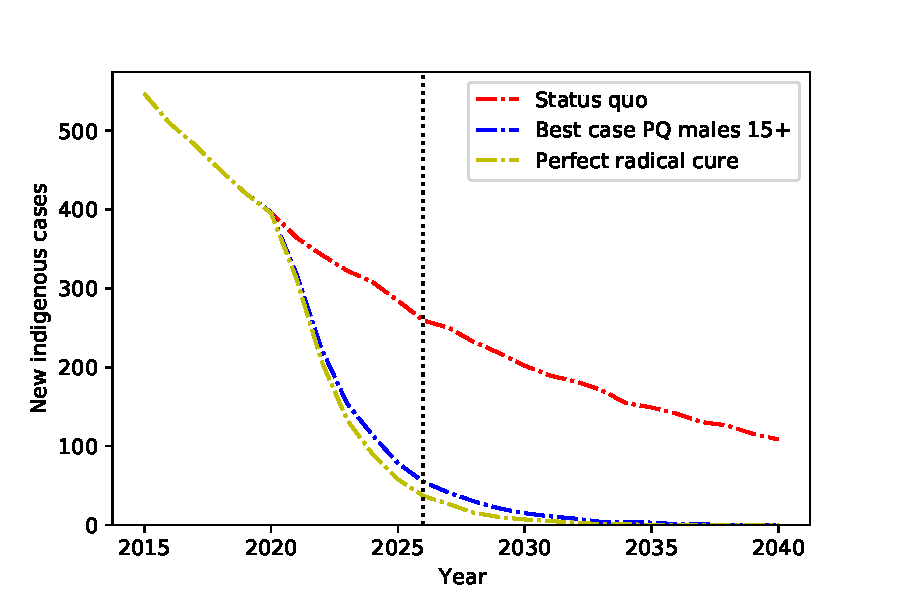
\includegraphics[width=.45\linewidth]{Pursat_low_indigenous_cases_Total.pdf}} 
\subcaptionbox{Total, low.\label{Pursat_low_active_cases_Total}}{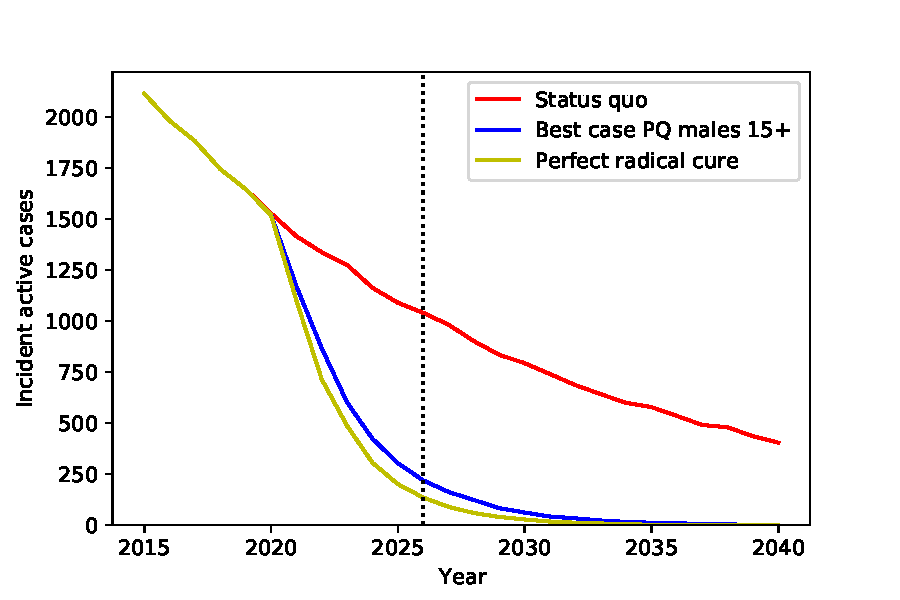
\includegraphics[width=.45\linewidth]{Pursat_low_active_cases_Total.pdf}} 
\caption{\csentence{\pq~intervention for \pv~in Pursat}. Lines represent annual medians for each individual year from 300 sampled model trajectories given the status quo and each radical cure scenario. Vertical dashed line is the December 2025 elimination target for \pv.}\label{fig:pq_Pursat}
\end{figure}

While the status quo scenario did not project \pv~elimination by 2025 in any provinces, the best case implementation of \pq~for \males~has a substantial impact on projected case numbers for \pv~in every province (Figure \ref{fig:pq_Pursat}, Table \ref{tab:radcure_numbers}). \pq~is not expected to result in achieving elimination by 2025 in more than 50\% of model trajectories in any province, but as seen in Table \ref{tab:radcure_percentage}, \pq~is projected to result in a 67\%--83\% reduction in \pv~case numbers by 2025. Conversely, the absence of a radical cure is projected to result in a continuation of calibrated trends prior to 2018, with a 1\%--14\% increase in case numbers by 2025 in the high baseline incidence scenarios, or a 23\%--37\% reduction in the low baseline incidence scenarios. In the high baseline incidence scenarios, a perfect radical cure able to be given to the entire population as treated for \pv~was estimated to result in \pv~elimination by 2040 in more than 50\% of model trajectories in Takeo and Pailin - the two lowest incidence provinces.

Figs~\ref{fig:elimination_low}--\ref{fig:elimination_high} show the proportion of model trajectories in which \pv~elimination was achieved by 2025, 2030, 2035, or 2040, given a baseline calibration to low or high historical estimates of incidence respectively. Over the longest time frame considered, best case \pq~increased the average proportion of model trajectories across provinces in which elimination was achieved in the high baseline incidence scenario by 2040 from 0\% to 26\%, or 42\% with a perfect radical cure. In the low baseline incidence scenario, best case \pq~increased the average proportion of model trajectories across provinces in which elimination was achieved by 2040 from 4\% to 70\%, or 77\% with a perfect radical cure.

\begin{figure}[h!]
\centering
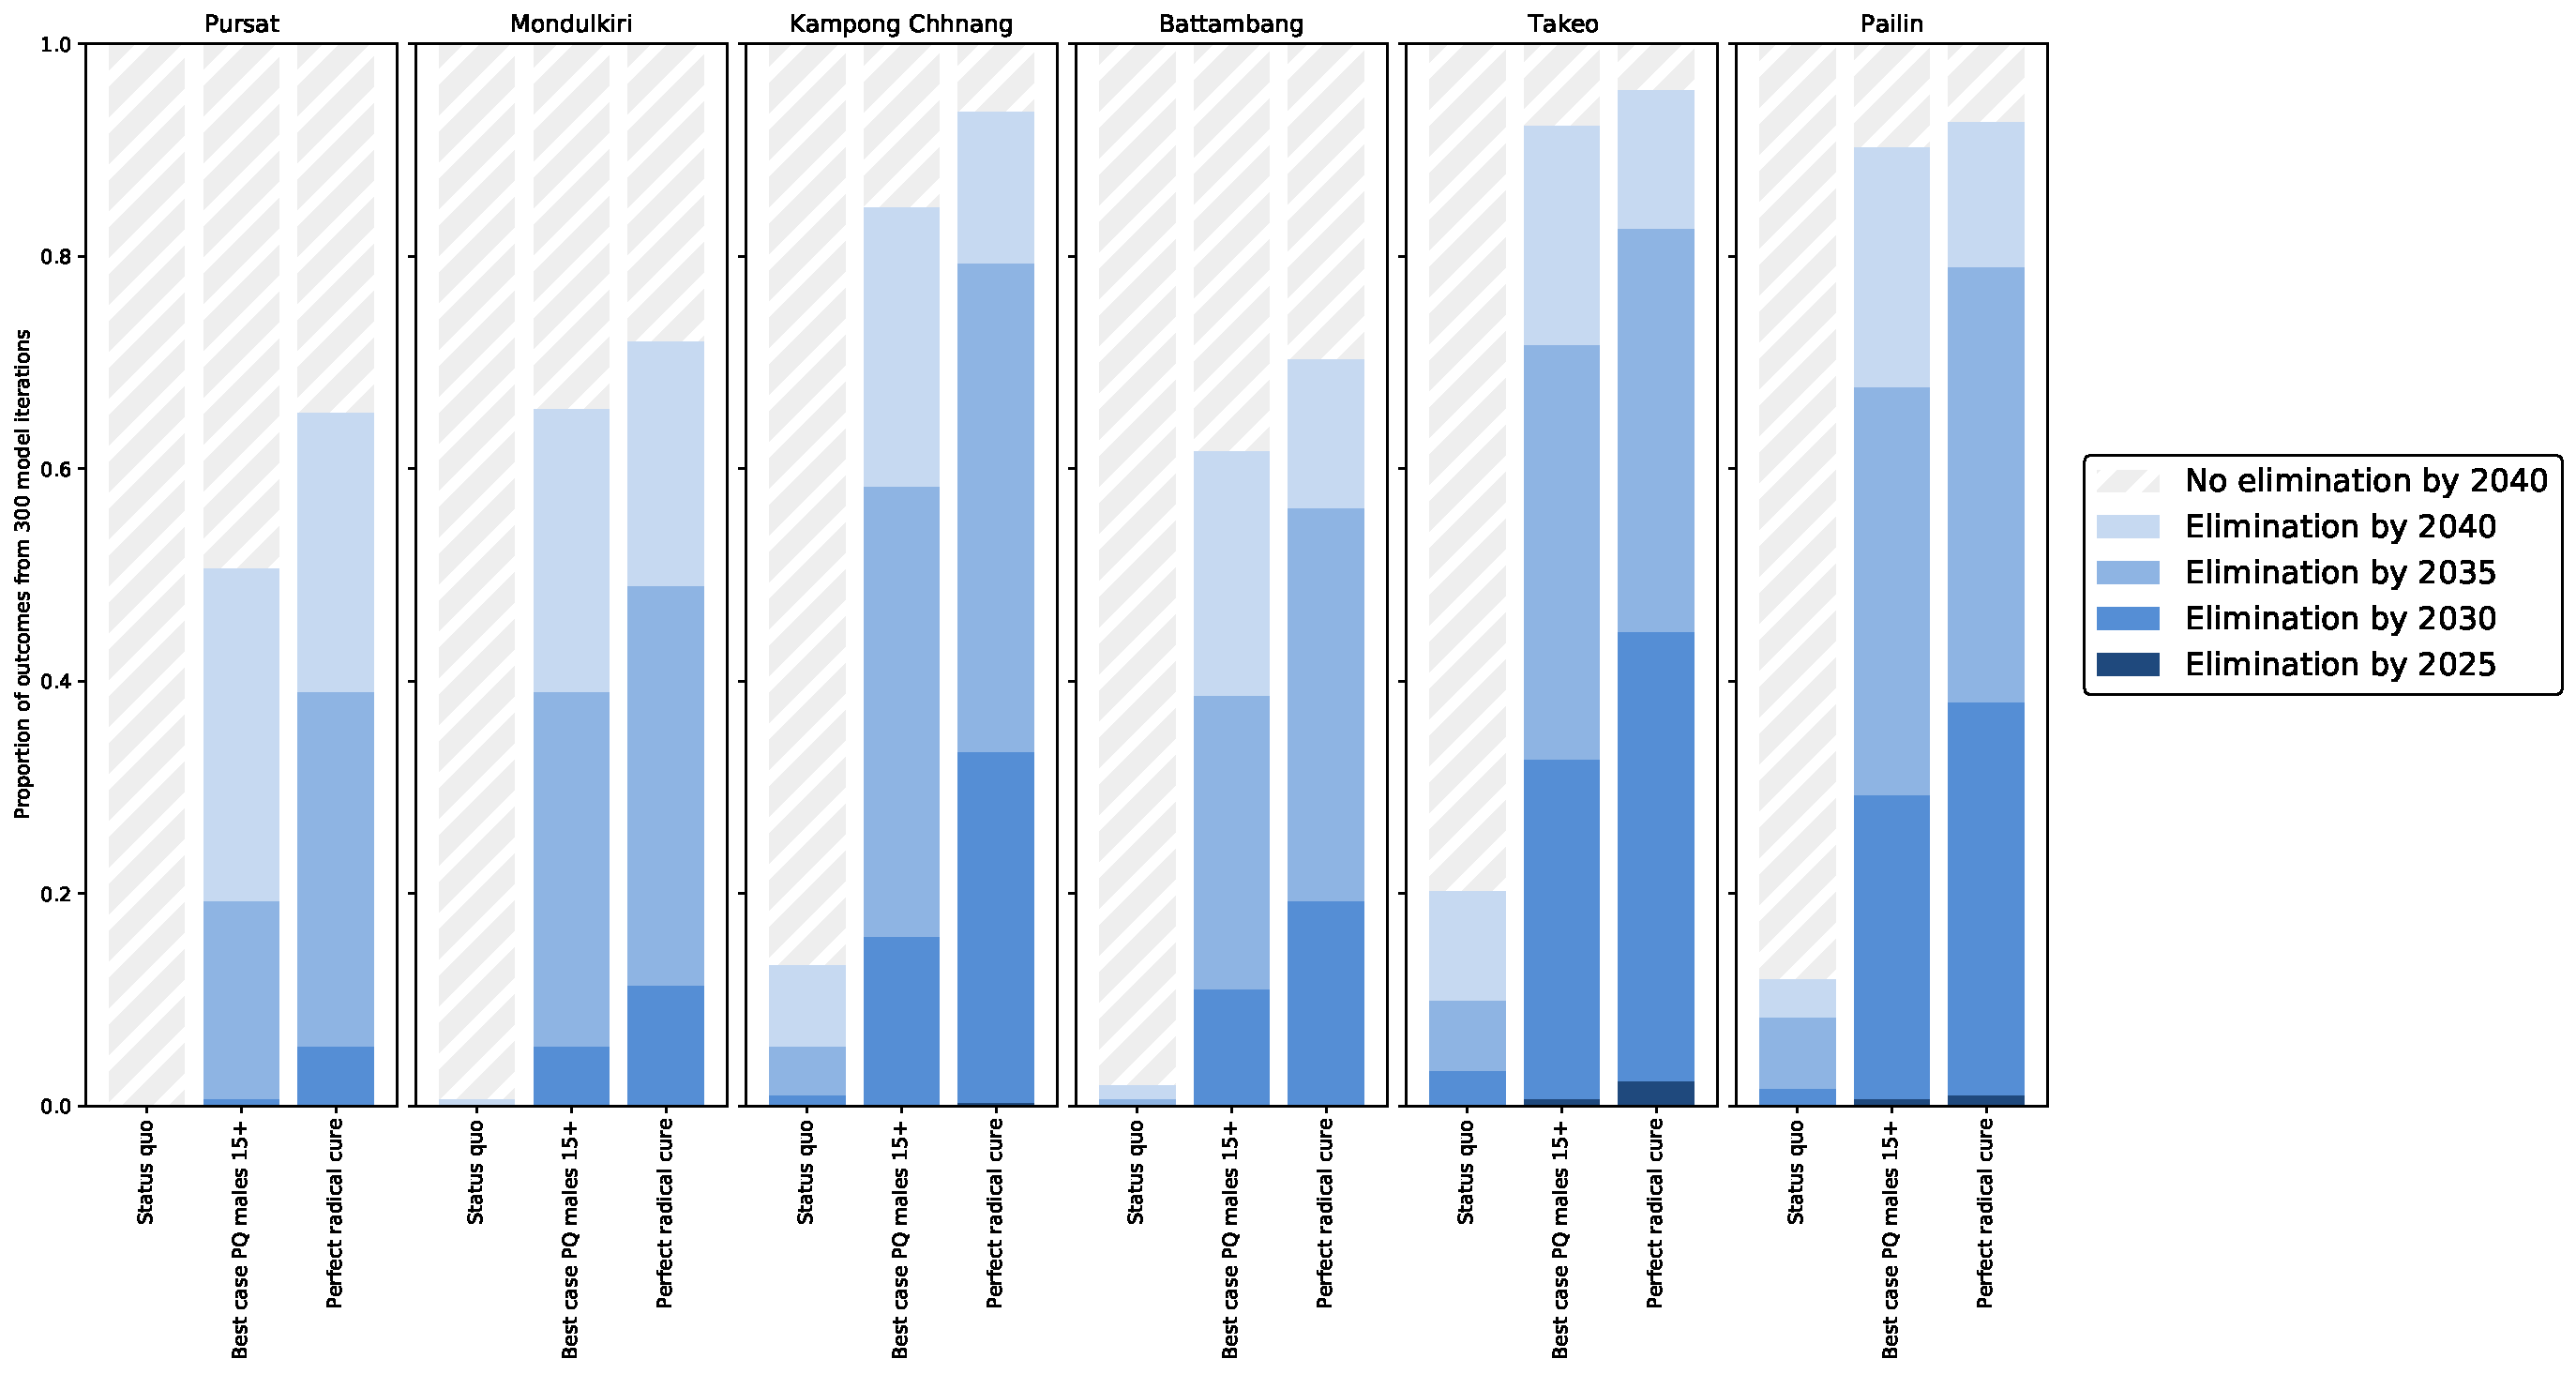
\includegraphics[width=0.95\linewidth]{low_baseline.pdf}
\caption{\csentence{Timing of elimination under low baseline incidence scenarios} of indigenous transmission of \pv, according to radical cure coverage achieved \pv. Proportions of 300 sampled model trajectories in which no indigenous \pv~transmission has occurred for a consecutive period of 3 years at any time prior to December 31 of that year.}\label{fig:elimination_low}
\end{figure}

\begin{figure}[h!]
\centering
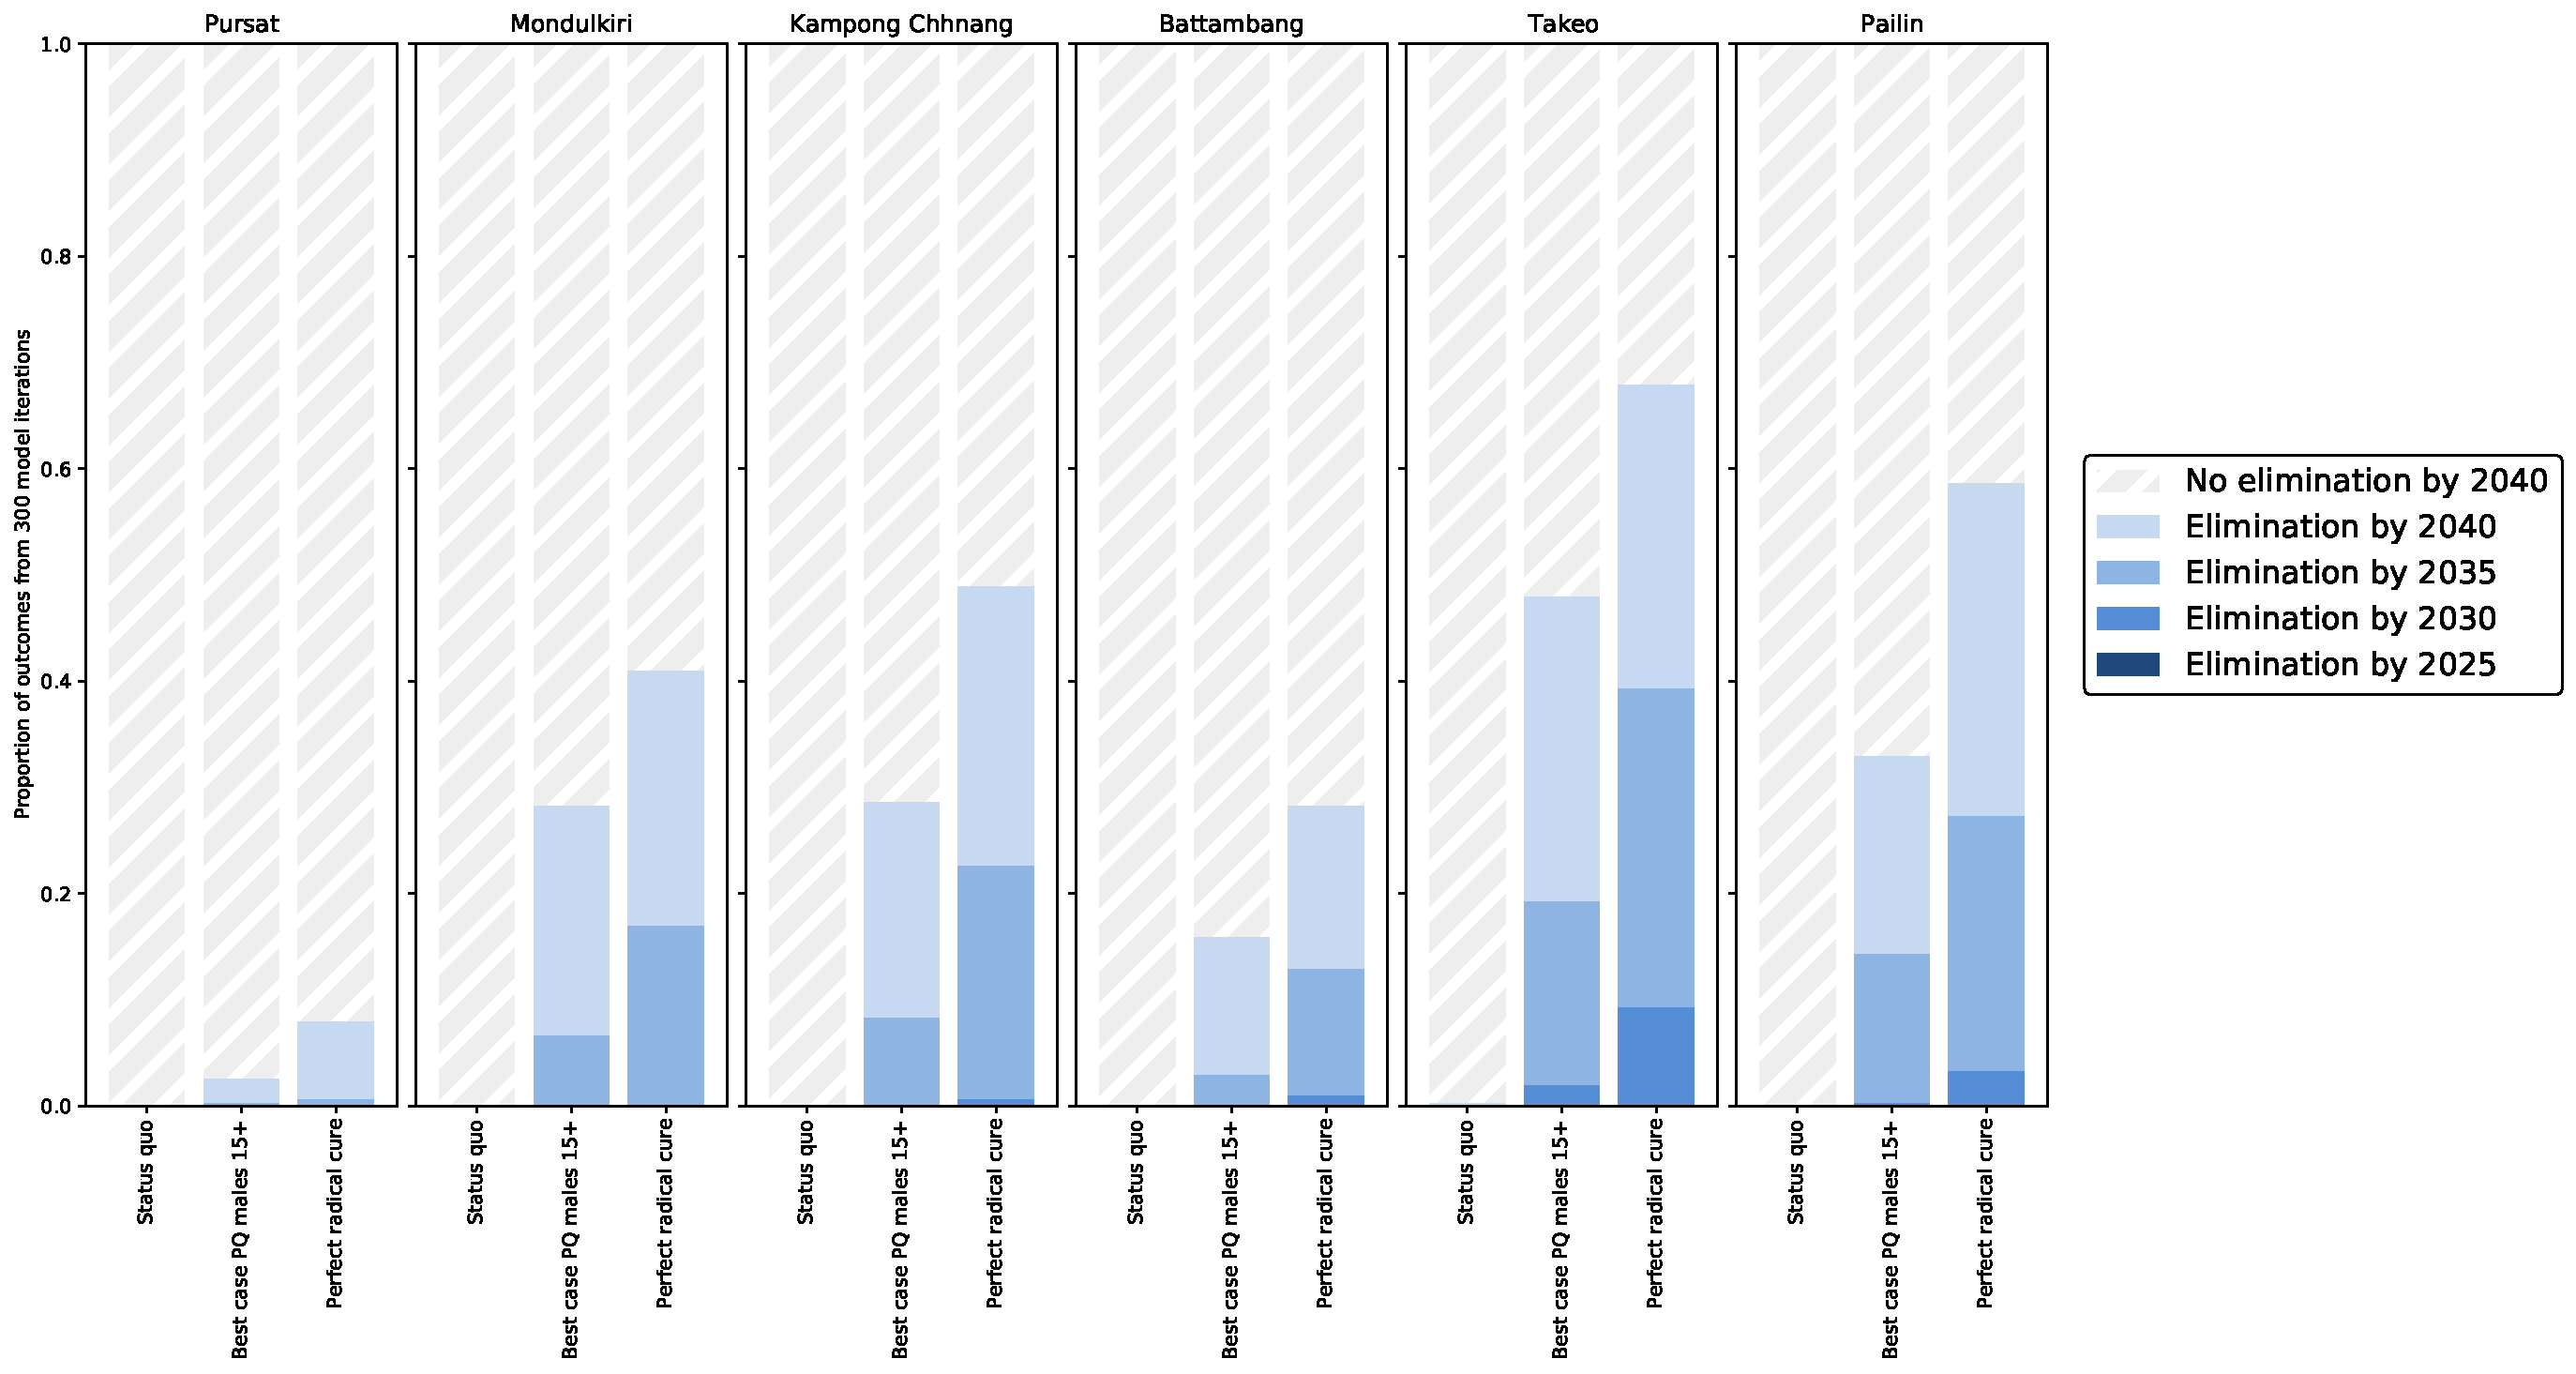
\includegraphics[width=0.95\linewidth]{high_baseline.pdf}
\caption{\csentence{Timing of elimination under high baseline incidence scenarios} of indigenous transmission of \pv, according to radical cure coverage achieved \pv. Proportions of 300 sampled model trajectories in which no indigenous \pv~transmission has occurred for a consecutive period of 3 years at any time prior to December 31 of that year.}\label{fig:elimination_high}
\end{figure}

%Discussion
%This section should discuss the implications of the findings in context of existing research and highlight limitations of the study.
\section*{Discussion}

% Statement of principal findings
We have used a transmission model to explore the potential impact of a \pq~radical cure (0.25 mg/kg daily x 14 days) for diagnosed \pv~cases in G6PD normal \males, which was a strategy Cambodia was considering for malaria elimination.  We found that this strategy is unlikely be sufficient to reach Cambodia's elimination target date of 2025 in any of the six provinces considered without additional novel interventions. The formal definition of elimination requires there to be no new indigenous transmission after 31 December 2022 in order to achieve three years without indigenous transmission by 31 December 2025 in line with the elimination target. Even under the most optimistic assumptions around baseline \pv~incidence, and beyond best case assumptions of expanded eligibility to all diagnosed \pv~cases and a 100\% efficacy radical cure, elimination was achieved by 2025 in less than 5\% of model trajectories in each province. If baseline incidence is in line with the low baseline incidence scenarios, then elimination by 2030 may be more feasible although still predicted to be achieved in less than 50\% of model trajectories in all provinces.

We have calibrated the Optima Malaria model for six provinces to include malaria interventions introduced prior to and during 2018 in Cambodia targeted primarily at earlier \pf~elimination, and the success that they also have at reducing indigenous transmission of \pv. However, without a \pq~radical cure, \pv~elimination was not predicted to be achieved even by 2040 in any model iteration in any province under the high baseline incidence scenarios, and not predicted to be achieved by 2040 in any model trajectories for Pursat, or Mondulkiri under the low baseline incidence scenario, with the remaining provinces achieving elimination by 2040 in less than 20\% of model trajectories. Without wide-scale implementation of a radical cure, \pv~is projected to continue in each province of Cambodia.

Conversely, even though we projected that elimination by 2025 would only be achieved in a small minority of model trajectories, elimination over the longer-term appears to be feasible if a \pq~intervention for \males~can be sustained. Because the majority of \pv~cases are in \males, this best case intervention has qualitatively similar success rates under the low baseline incidence scenarios in achieving elimination by 2040 as a hypothetical perfect radical cure.

%If the high baseline incidence scenarios better match trends as new incidence data becomes available, achieving high coverage of \pq~for all those eligible will be more critical, and additional or emerging interventions may be necessary to achieve \pv~elimination in Cambodia. 



% Strengths and weaknesses in relation to other studies, discussing particularly any differences in results
%While there are other \pv~transmission models, 
As far as we are aware, there have been no other modelling studies answering the question of elimination of \pv~through a \pq~intervention for G6PD normal \males~in Cambodia. The transmission model used here contains the flexibility to define the minimal necessary populations and stages of malaria to answer the question posed about reaching elimination by the target date. Furthermore, the Optima Malaria model can be used to evaluate optimal resource allocation to \pv~-targeting malaria interventions as has been applied to \pf~previously~\cite{scott2017}.

% Strengths and weaknesses of the study
We have calibrated models for \pv~transmission for six provinces in Cambodia, to high and low baseline incidence scenarios to capture the reasonable bounds of uncertainty arising from limited data and changes in surveillance methods and interventions between 2011 and 2018. By including both a ``best case'' and a far beyond best case scenario for the implementation of a \pq~radical cure, our approach increases confidence in our answer to the posed question: \pv~is not likely to be eliminated by the target date of 2025 in Cambodia through the use of \pq~in addition to 2018 status quo interventions for \males~or even with all populations being eligible. The actual impact under real-world conditions is likely to include lower values for each of coverage, eligibility, and effectiveness as demonstrated in the trial implementation \cite{brief_g6pdtests_2020} where 29.6\%  of eligible \males~completed a radical cure compared with the ``best case'' value of 71\% evaluated here, or 100\% in the perfect radical cure scenario.

% Meaning of the study: possible mechanisms and implications for clinicians or policymakers
Future updates to incidence estimates \cite{ngor2018} and inclusion of the population-targeted activities and routine use of malaria surveillance data already put into practice by the CNM as part of an ``Intensification Plan'' which has resulted in reported \pf/mixed cases declining by 97.4\% between October 2018 and December 2020 \cite{sovannaroth2022accelerating} may reduce the uncertainty interval from sampled model baselines. As Cambodia now seeks to continue progress in reaching malaria elimination targets, modelling of the combined impact of \pq~with other ``last mile'' interventions could further enhance targeting. 

%Conclusions
%This should state clearly the main conclusions and provide an explanation of the importance and relevance of the study reported.
\section*{Conclusions}

We have used transmission modelling to answer a key question for Cambodia posed prior to the implementation of the wider intensification of elimination efforts: will the use of a \pq~radical cure (0.25 mg/kg daily x 14 days) for diagnosed \pv~cases in G6PD normal \males~from October 2020, in addition to 2018 status quo interventions, be sufficient to eliminate \textit{Plasmodium vivax} by the target date of 2025. Given the uncertainties in the case data, we have used a best case scenario approach. We found \pv~is not likely to be eliminated by any province by the target date. However, \pq~remains a critical intervention, as the absence of a radical cure means \pv~elimination is unlikely to be achieved in this setting over any time frame. \pq~is projected by this model to have a substantial impact, on both blood stage infections (clinical and asymptomatic), and hypnozoite reservoirs. While \pq~alone may not result in elimination of \pv~by the target date, we project that sustained application of effective \pq~may result in the elimination of \pv~by 2040 or earlier, and this evidence may help guide the need for either additional interventions or a change in target date.

%List of abbreviations
%If abbreviations are used in the text they should be defined in the text at first use, and a list of abbreviations should be provided.
\section*{List of abbreviations}

\begin{table}[h]
    \centering
    \begin{tabular}{r l}
        CNM & Cambodia National Center for Parasitology, Entomology and Malaria Control \\
        \pv & \textit{Plasmodium vivax} \\
        \pf & \textit{Plasmodium falciparum} \\
        CQ & Chloroquine \\
        PQ & Primaquine \\
        \males & Males, 15 years of age and older \\
        \gen & Females, 15 years of age and older, and all children under 15 years \\ 
    \end{tabular}
    %\caption{Caption}
    \label{tab:abbreviations}
\end{table}



%%%%%%%%%%%%%%%%%%%%%%%%%%%%%%%%%%%%%%%%%%%%%%
%%                                          %%
%% Backmatter begins here                   %%
%%                                          %%
%%%%%%%%%%%%%%%%%%%%%%%%%%%%%%%%%%%%%%%%%%%%%%

\begin{backmatter}

\section*{Availability of data and materials}
National malaria surveillance data available at \url{https://mis.cnm.gov.kh/}. The aggregated data used to conduct this analysis, as well as the code used to run the model and generate results are available on GitHub at \url{https://github.com/rihickson/vivax-primaquine-Cambodia}. 

\section*{Competing interests}
  The authors declare that they have no competing interests.

\section*{Author's contributions}
    PN, RIH, RMH, AD, DJP, and JMM conceived of the project and oversaw the design. PN and RIH curated the data. RMH, RIH, and RA developed the transmission model and code implementation, and calibrated the model. RIH, DJP, JMM wrote the surveillance decision support model. RIH, RMH, DJP, AD, JAS, FJIF, NS, JMM, PN prepared the manuscript. All authors read and approved the final manuscript.

\section*{Acknowledgements}
This work is supported in part by the Australian Centre for Research Excellence in Malaria Elimination, funded by the NHMRC (1134989). JAS is funded by an Australian National Health and Medical Research Council of Australia (NHMRC) Investigator Grant (1196068) and FJIF by a NHMRC Career Development Fellowship (1166753).

%%%%%%%%%%%%%%%%%%%%%%%%%%%%%%%%%%%%%%%%%%%%%%%%%%%%%%%%%%%%%
%%                  The Bibliography                       %%
%%                                                         %%
%%  Bmc_mathpys.bst  will be used to                       %%
%%  create a .BBL file for submission.                     %%
%%  After submission of the .TEX file,                     %%
%%  you will be prompted to submit your .BBL file.         %%
%%                                                         %%
%%                                                         %%
%%  Note that the displayed Bibliography will not          %%
%%  necessarily be rendered by Latex exactly as specified  %%
%%  in the online Instructions for Authors.                %%
%%                                                         %%
%%%%%%%%%%%%%%%%%%%%%%%%%%%%%%%%%%%%%%%%%%%%%%%%%%%%%%%%%%%%%

% if your bibliography is in bibtex format, use those commands:
\bibliographystyle{bmc-mathphys} % Style BST file (bmc-mathphys, vancouver, spbasic).
\bibliography{bmc_article}      % Bibliography file (usually '*.bib' )
% for author-year bibliography (bmc-mathphys or spbasic)
% a) write to bib file (bmc-mathphys only)
% @settings{label, options="nameyear"}
% b) uncomment next line
%\nocite{label}

% or include bibliography directly:
% \begin{thebibliography}
% \bibitem{b1}
% \end{thebibliography}

%%%%%%%%%%%%%%%%%%%%%%%%%%%%%%%%%%%
%%                               %%
%% Figures                       %%
%%                               %%
%% NB: this is for captions and  %%
%% Titles. All graphics must be  %%
%% submitted separately and NOT  %%
%% included in the Tex document  %%
%%                               %%
%%%%%%%%%%%%%%%%%%%%%%%%%%%%%%%%%%%

%%
%% Do not use \listoffigures as most will included as separate files

%\section*{Figures}
%  \begin{figure}[h!]
%  \caption{\csentence{Model calibration for Mondulkiri.}
%      Number of malaria cases as a function of time, from 2011 to 2025. A) General population for the high and increasing baseline incidence. B) Males 15 years and older population for the high and increasing baseline incidence. C) General population for the low and decreasing baseline incidence. D) Males 15 years and older population for the low and decreasing baseline incidence. }
%      \end{figure}
%
%\begin{figure}[h!]
%  \caption{\csentence{Sample figure title.}
%      Figure legend text.}
%      \end{figure}



%%%%%%%%%%%%%%%%%%%%%%%%%%%%%%%%%%%
%%                               %%
%% Tables                        %%
%%                               %%
%%%%%%%%%%%%%%%%%%%%%%%%%%%%%%%%%%%

%% Use of \listoftables is discouraged.
%%
%%\section*{Tables}
%%\begin{table}[p] 
%%\caption{Surveillance targets for 0.99 probability of detecting at least one case of \pv~in a province, given the scenarios outlined in \S~\ref{sec:methods}, assuming 100\% sensitivity and specificity of the tests (so a lower bound on number of targets).}\label{tab:surveillance}
%%      \begin{tabular}{|l|l|l|l|l|l|l|l|l|l|}
%%       \hline 
%%       \multicolumn{2}{|l|}{Year} & \multicolumn{4}{|c|}{2020} & \multicolumn{4}{|c|}{2025} \\ \hline
%%       \multirow{2}{*}{Scenario} & Incidence & Low & Low & High & High & Low & Low & High & High \\ %\hline 
%%                                 & Primaquine & None & M 15+ & None & M 15+ & None & M 15+ & None & M 15+ \\ \hline
%%    \multirow{6}{*}{Province} & Pursat & 441 & 444 & 2,345 & 76 & 76 & 557 & 2,610 & 70 \\ %\hline
%%Mondulkiri & 172 & 173 & 48 & 48 & 280 & 1,388 & 54 & 263 \\ %\hline
%%                              & Kampong Chhnang & 3,798 & 3,819 & 649 & 653 & 5,564 & 26,094 & 614 & 2,998 \\ %\hline 
%%                              & Battambang & 2,962 & 2,978 & 433 & 436 & 3,916 & 19,191 & 384 & 1,922 \\ %\hline
%%                              & Pailin & 850 & 855 & 123 & 124 & 1,040 & 4,960 & 122 & 579 \\ %\hline 
%%                              & Takeo & 14,335 & 14,415 & 2,345 & 2,358 & 18,905 & 89,418 & 2,205 & 10,919 \\ \hline 
%%      \end{tabular}
%%\end{table}

%%%%%%%%%%%%%%%%%%%%%%%%%%%%%%%%%%%
%%                               %%
%% Additional Files              %%
%%                               %%
%%%%%%%%%%%%%%%%%%%%%%%%%%%%%%%%%%%

\section*{Additional Files}\label{supp}
Detailed descriptions of the model, data, and calibration are provided in the Supplementary appendix. 
%  \subsection*{Additional file 1 --- Sample additional file title}
%    Additional file descriptions text (including details of how to
%    view the file, if it is in a non-standard format or the file extension).  This might
%    refer to a multi-page table or a figure.
%
%  \subsection*{Additional file 2 --- Sample additional file title}
%    Additional file descriptions text.

% \subsection*{Additional file 1 --- Model and data details}
%     Detailed descriptions of the model and data are provided here, including supplementary figures with a further breakdown on the modelled impact. 

\begin{figure}[h!]
\centering
\subcaptionbox{Males 15+.\label{calibration_Mondul_Kiri_active_cases_M}}{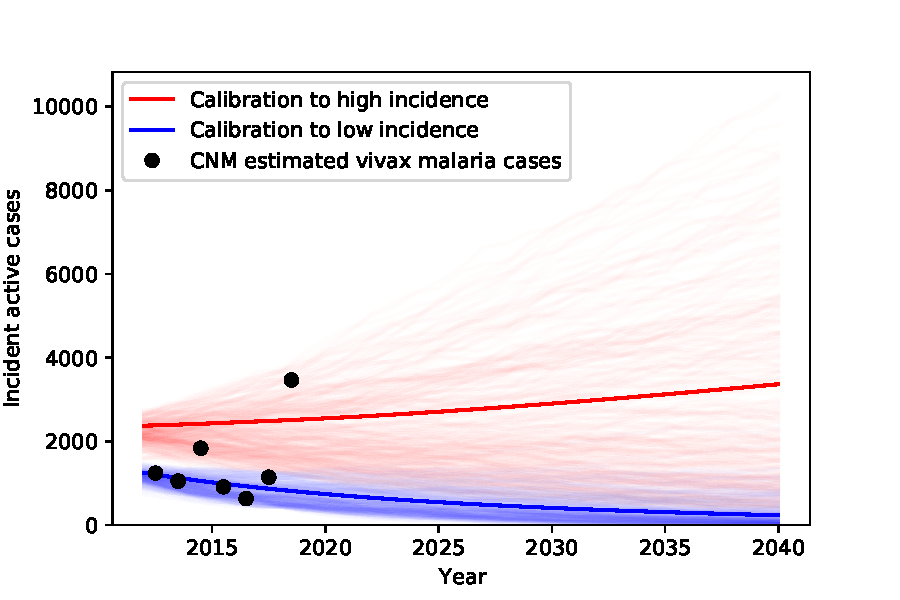
\includegraphics[width=.45\linewidth]{calibration_Mondul_Kiri_active_cases_M 15+.pdf}} 
\subcaptionbox{Gen, low.\label{calibration_Mondul_Kiri_active_cases_Gen}}{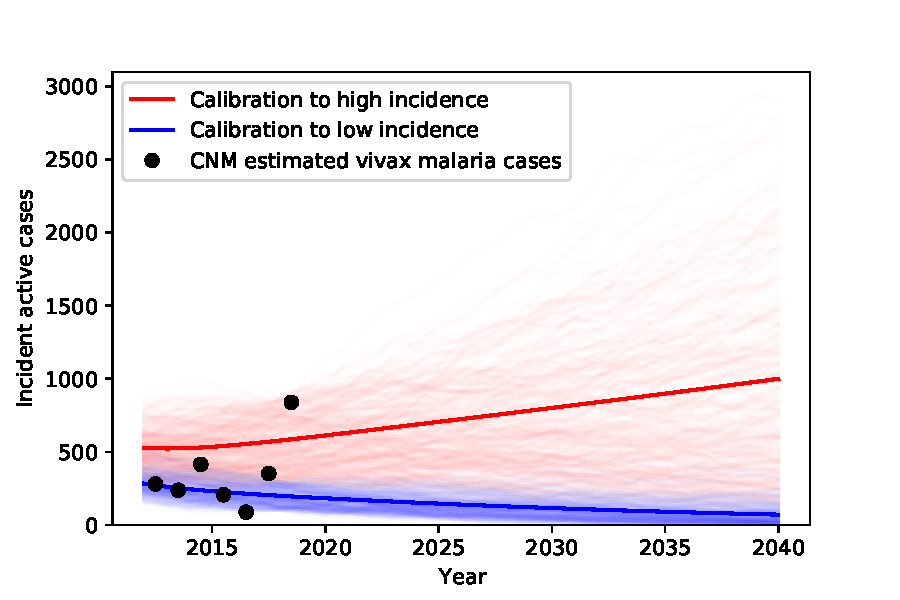
\includegraphics[width=.45\linewidth]{calibration_Mondul_Kiri_active_cases_Gen.pdf}} 
\caption{\csentence{Calibration to reported \pv~cases in Mondulkiri.} Faint lines represent sampled model trajectories for each of the low and high incidence calibrations.}\label{fig:calibration_Mondulkiri}
\end{figure}

\begin{figure}[h!]
\centering
\subcaptionbox{Males 15+.\label{calibration_Kampong_Chhnang_active_cases_M}}{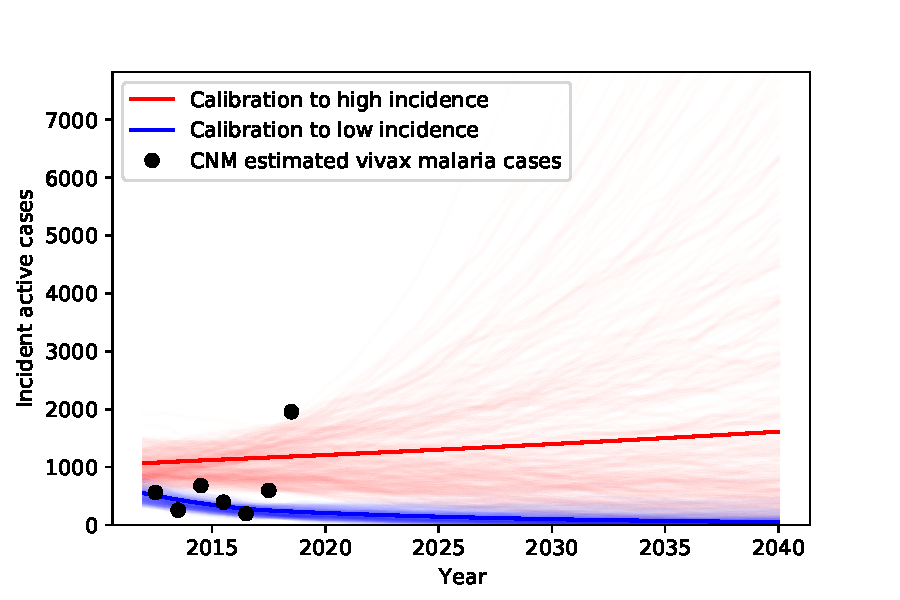
\includegraphics[width=.45\linewidth]{calibration_Kampong_Chhnang_active_cases_M 15+.pdf}} 
\subcaptionbox{Females 15+ and children.\label{calibration_Kampong_Chhnang_active_cases_Gen}}{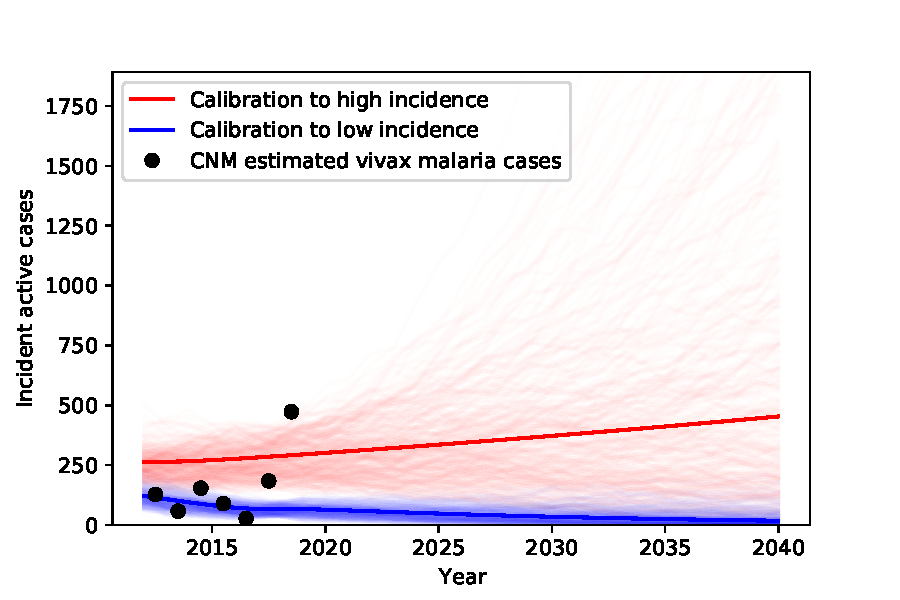
\includegraphics[width=.45\linewidth]{calibration_Kampong_Chhnang_active_cases_Gen.pdf}} 
\caption{\csentence{Calibration to reported \pv~cases in Kampong Chhnang.} Faint lines represent sampled model trajectories for each of the low and high incidence calibrations.}\label{fig:calibration_Kampong_Chhnang}
\end{figure}

\begin{figure}[h!]
\centering
\subcaptionbox{Males 15+.\label{calibration_Battambang_active_cases_M}}{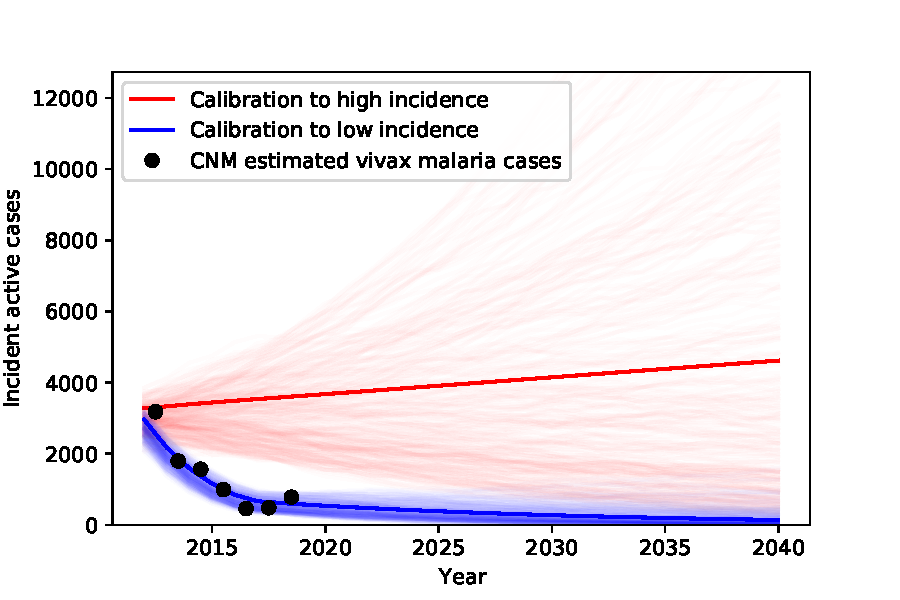
\includegraphics[width=.45\linewidth]{calibration_Battambang_active_cases_M 15+.pdf}} 
\subcaptionbox{Females 15+ and children.\label{calibration_Battambang_active_cases_Gen}}{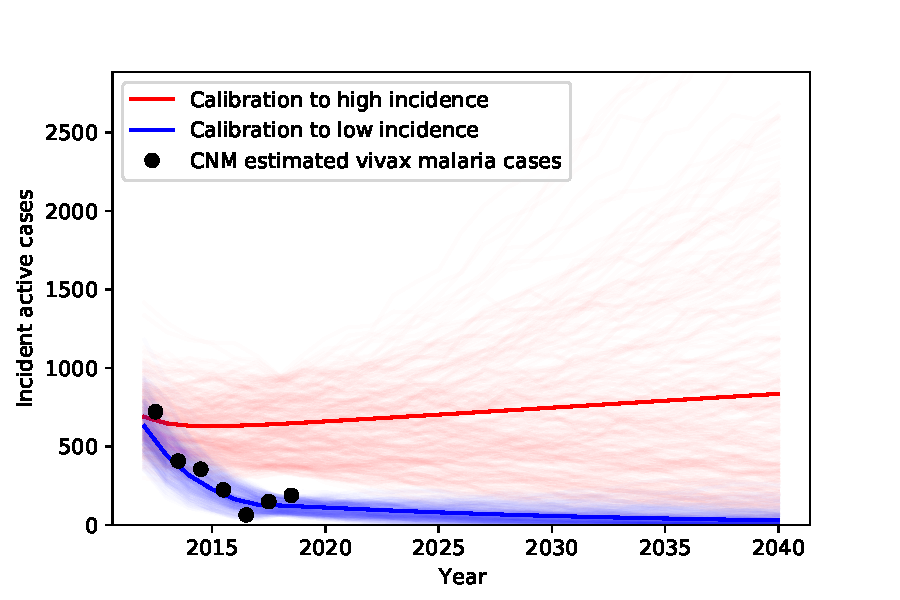
\includegraphics[width=.45\linewidth]{calibration_Battambang_active_cases_Gen.pdf}} 
\caption{\csentence{Calibration to reported \pv~cases in Battambang.} Faint lines represent sampled model trajectories for each of the low and high incidence calibrations.}\label{fig:calibration_Battambang}
\end{figure}

\begin{figure}[h!]
\centering
\subcaptionbox{Males 15+.\label{calibration_Takeo_active_cases_M}}{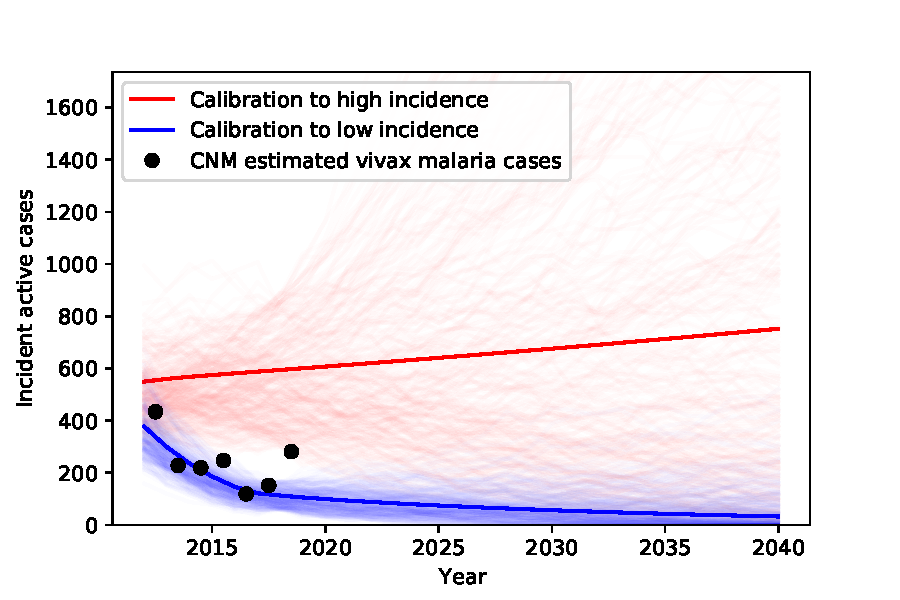
\includegraphics[width=.45\linewidth]{calibration_Takeo_active_cases_M 15+.pdf}} 
\subcaptionbox{Females 15+ and children.\label{calibration_Takeo_active_cases_Gen}}{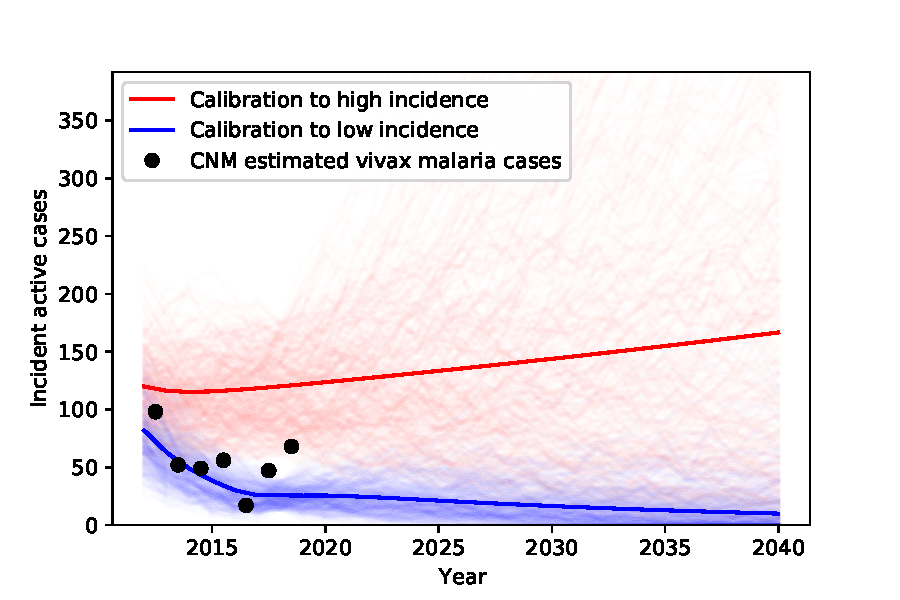
\includegraphics[width=.45\linewidth]{calibration_Takeo_active_cases_Gen.pdf}} 
\caption{\csentence{Calibration to reported \pv~cases in Takeo.} Faint lines represent sampled model trajectories for each of the low and high incidence calibrations.}\label{fig:calibration_Takeo}
\end{figure}

\begin{figure}[h!]
\centering
\subcaptionbox{Males 15+.\label{calibration_Pailin_active_cases_M}}{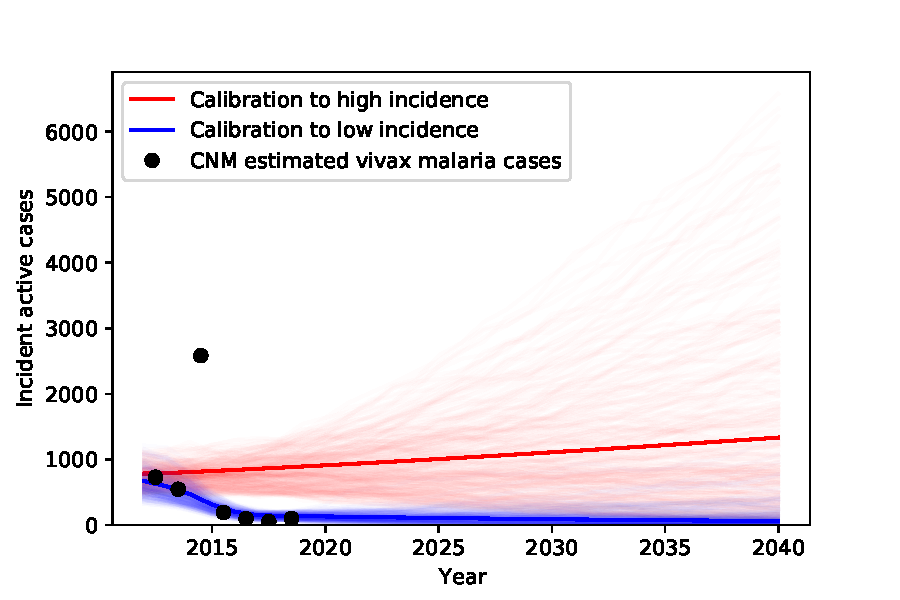
\includegraphics[width=.45\linewidth]{calibration_Pailin_active_cases_M 15+.pdf}} 
\subcaptionbox{Females 15+ and children.\label{calibration_Pailin_active_cases_Gen}}{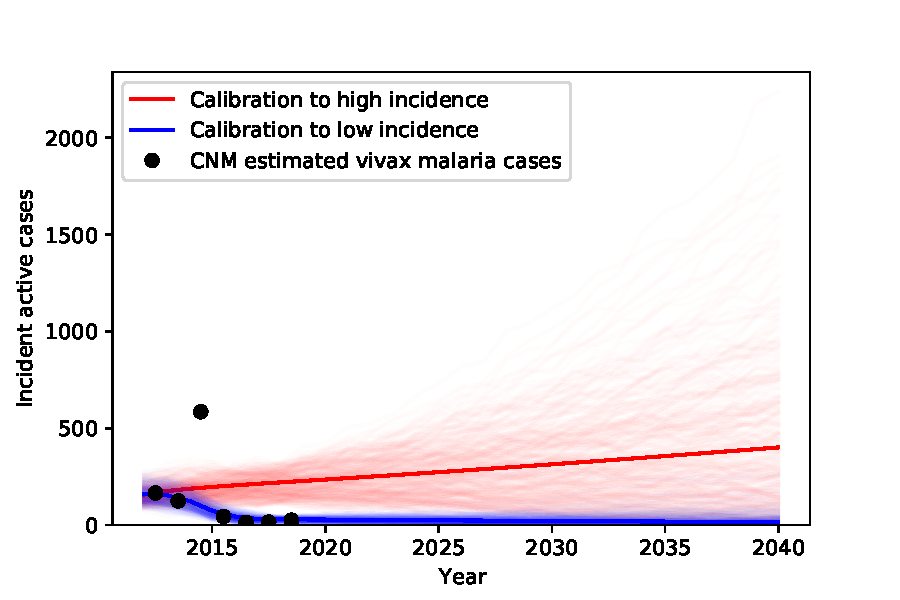
\includegraphics[width=.45\linewidth]{calibration_Pailin_active_cases_Gen.pdf}} 
\caption{\csentence{Calibration to reported \pv~cases in Pailin.} Faint lines represent sampled model trajectories for each of the low and high incidence calibrations.}\label{fig:calibration_Pailin}
\end{figure}

% -------------- PQ impact figs --------------
%---------------------------------------------
% --------------------------------------------


\begin{figure}[h!]
\centering
\subcaptionbox{Total, high.\label{Mondul_Kiri_high_indigenous_cases_Total}}{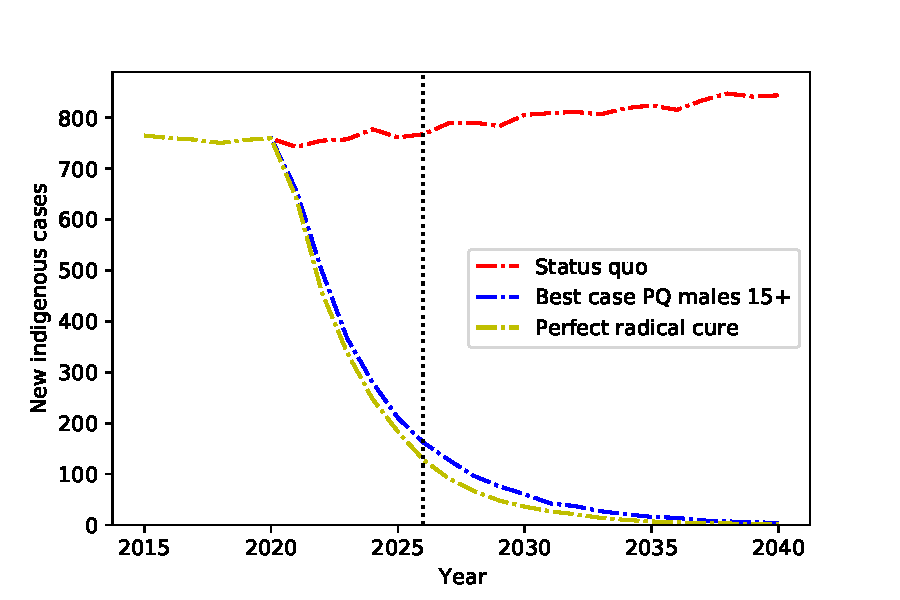
\includegraphics[width=.45\linewidth]{Mondul_Kiri_high_indigenous_cases_Total.pdf}} 
\subcaptionbox{Total, high.\label{Mondul_Kiri_high_active_cases_Total}}{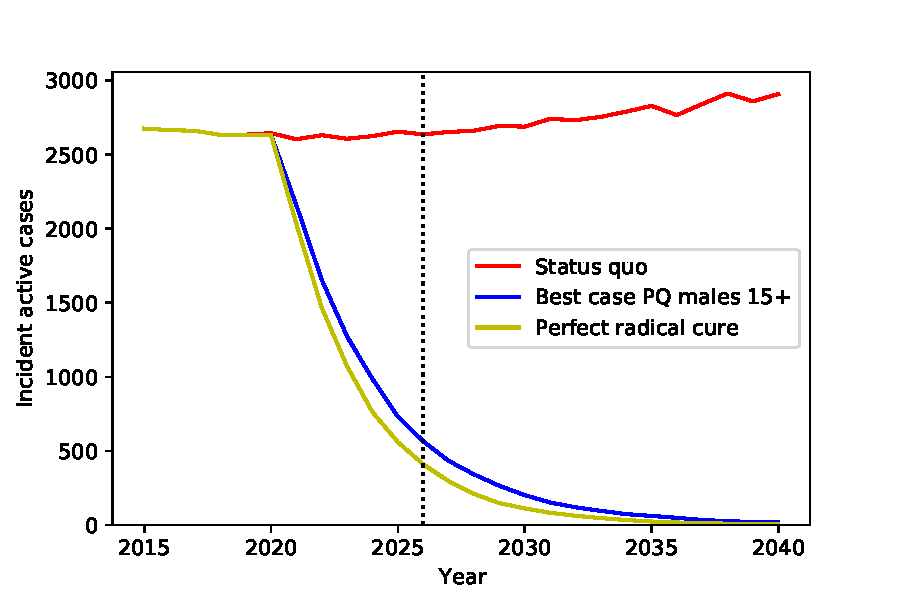
\includegraphics[width=.45\linewidth]{Mondul_Kiri_high_active_cases_Total.pdf}} 
\subcaptionbox{Total, low.\label{Mondul_Kiri_low_indigenous_cases_Total}}{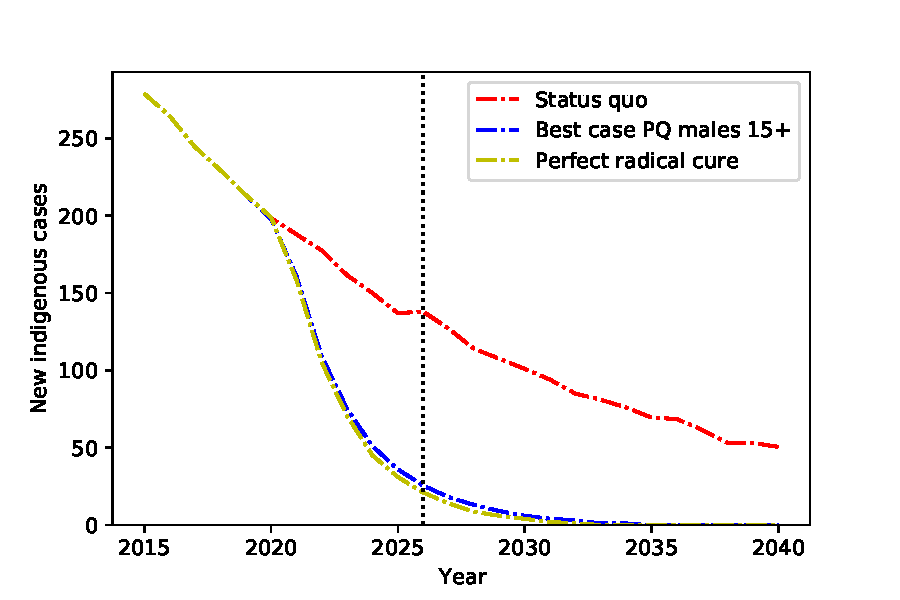
\includegraphics[width=.45\linewidth]{Mondul_Kiri_low_indigenous_cases_Total.pdf}} 
\subcaptionbox{Total, low.\label{Mondul_Kiri_low_active_cases_Total}}{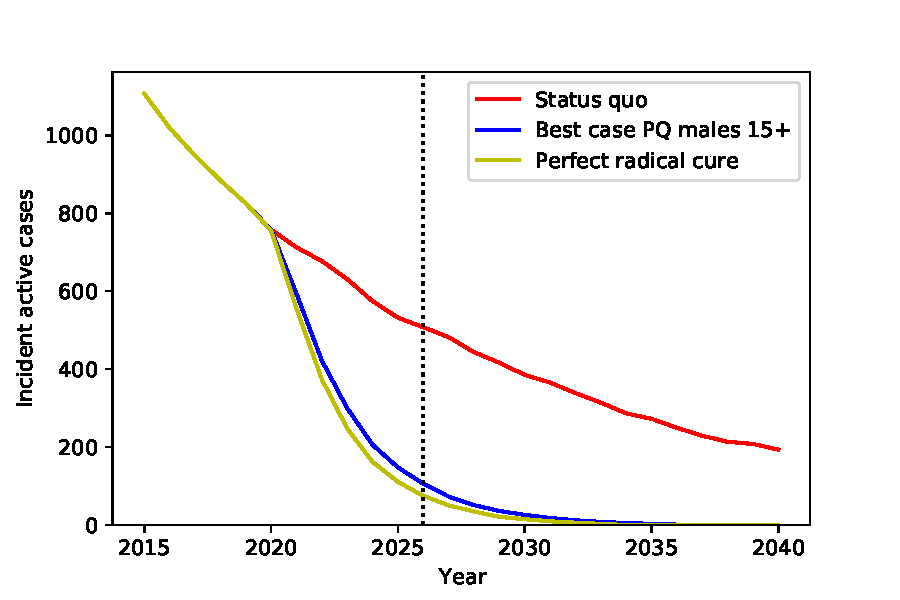
\includegraphics[width=.45\linewidth]{Mondul_Kiri_low_active_cases_Total.pdf}} 
\caption{\small \csentence{\pq~intervention for \pv~in Mondulkiri}. Lines represent annual medians for each individual year from 300 sampled model trajectories given the status quo and each radical cure scenario. Vertical dashed line is the December 2025 elimination target for \pv.}\label{fig:pq_Mondulkiri}
\end{figure}

\begin{figure}[h!]
\centering
\subcaptionbox{Total, high.\label{Kampong_Chhnang_high_indigenous_cases_Total}}{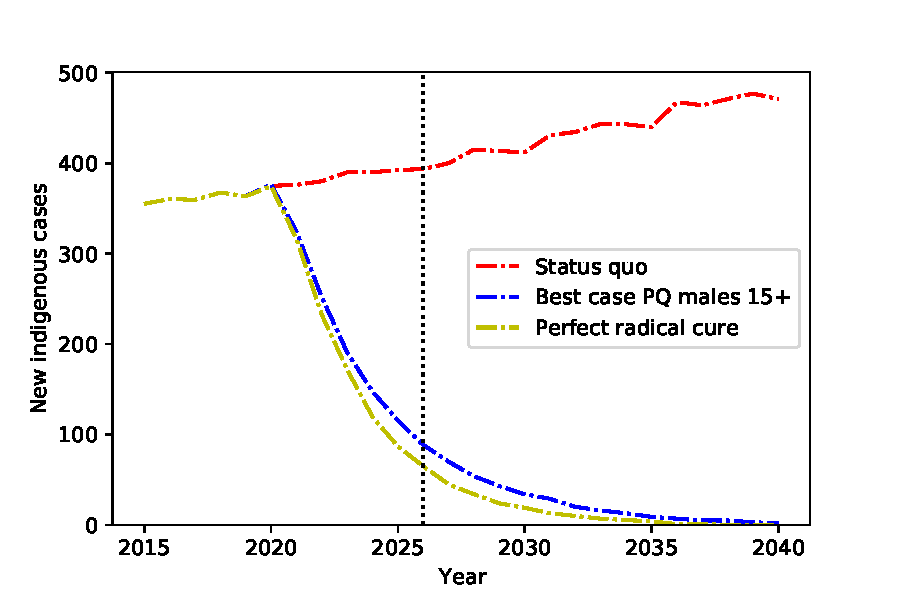
\includegraphics[width=.45\linewidth]{Kampong_Chhnang_high_indigenous_cases_Total.pdf}} 
\subcaptionbox{Total, high.\label{Kampong_Chhnang_high_active_cases_Total}}{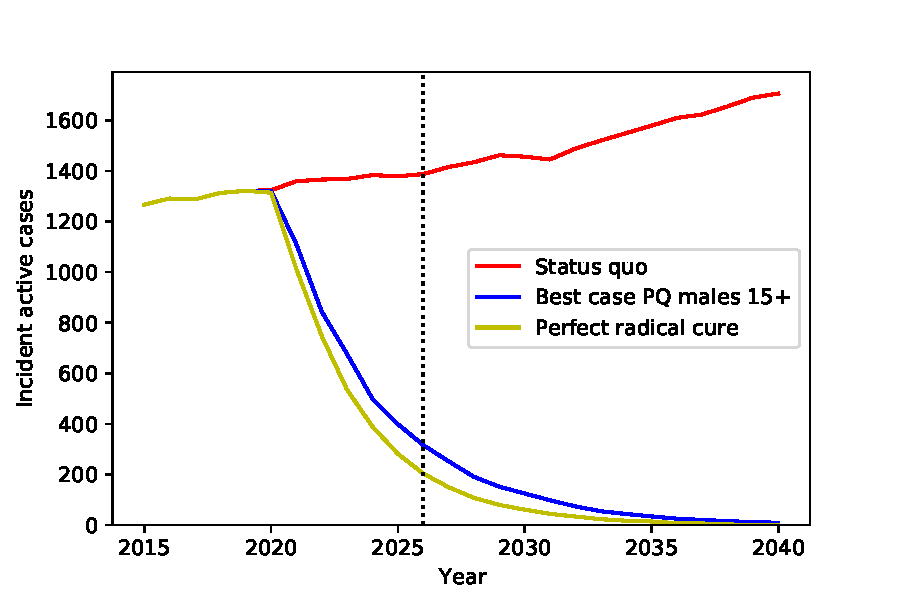
\includegraphics[width=.45\linewidth]{Kampong_Chhnang_high_active_cases_Total.pdf}} 
\subcaptionbox{Total, low.\label{Kampong_Chhnang_low_indigenous_cases_Total}}{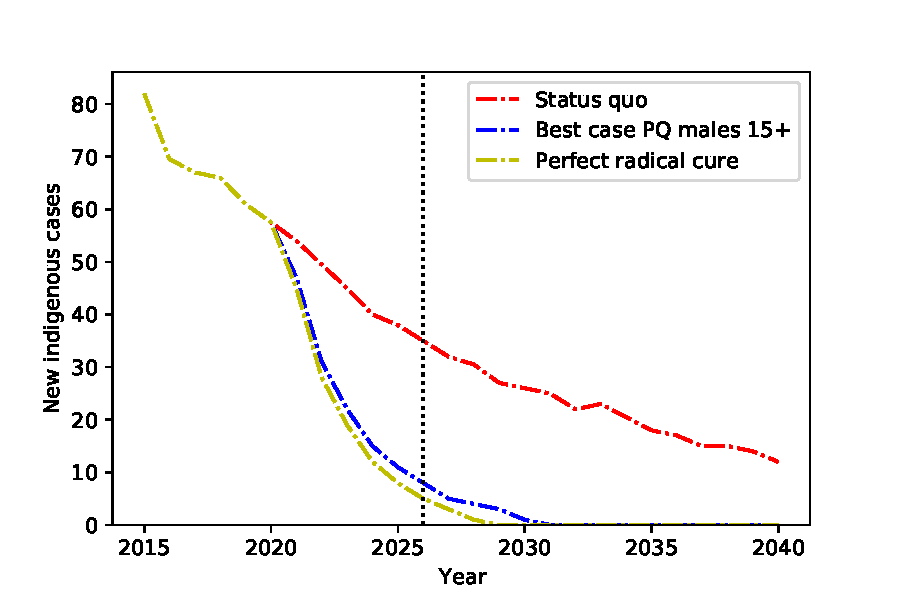
\includegraphics[width=.45\linewidth]{Kampong_Chhnang_low_indigenous_cases_Total.pdf}} 
\subcaptionbox{Total, low.\label{Kampong_Chhnang_low_active_cases_Total}}{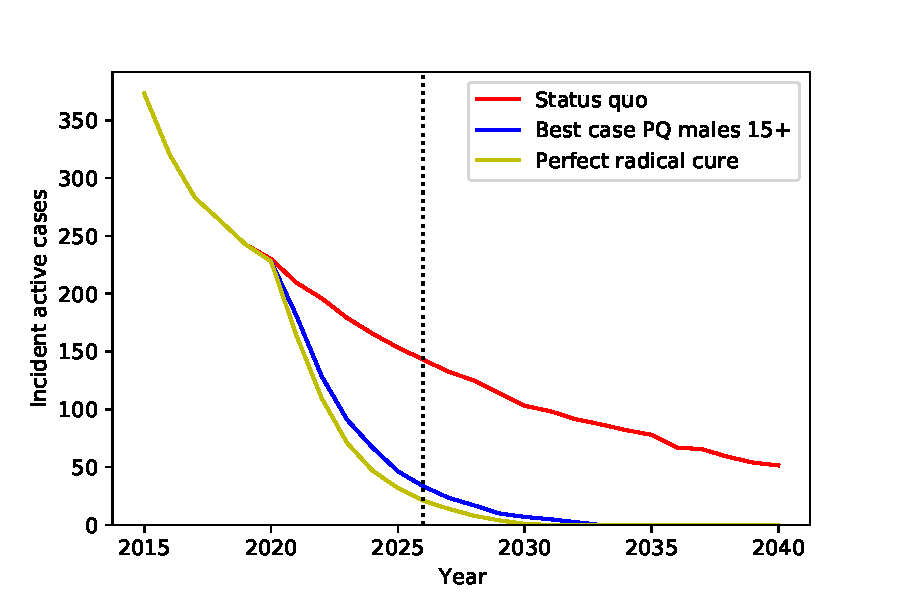
\includegraphics[width=.45\linewidth]{Kampong_Chhnang_low_active_cases_Total.pdf}} 
\caption{\small \csentence{\pq~intervention for \pv~in Kampong Chhnang}. Lines represent annual medians for each individual year from 300 sampled model trajectories given the status quo and each radical cure scenario. Vertical dashed line is the December 2025 elimination target for \pv.}\label{fig:pq_Kampong_Chhnang}
\end{figure}

\begin{figure}[h!]
\centering
\subcaptionbox{Total, high.\label{Battambang_high_indigenous_cases_Total}}{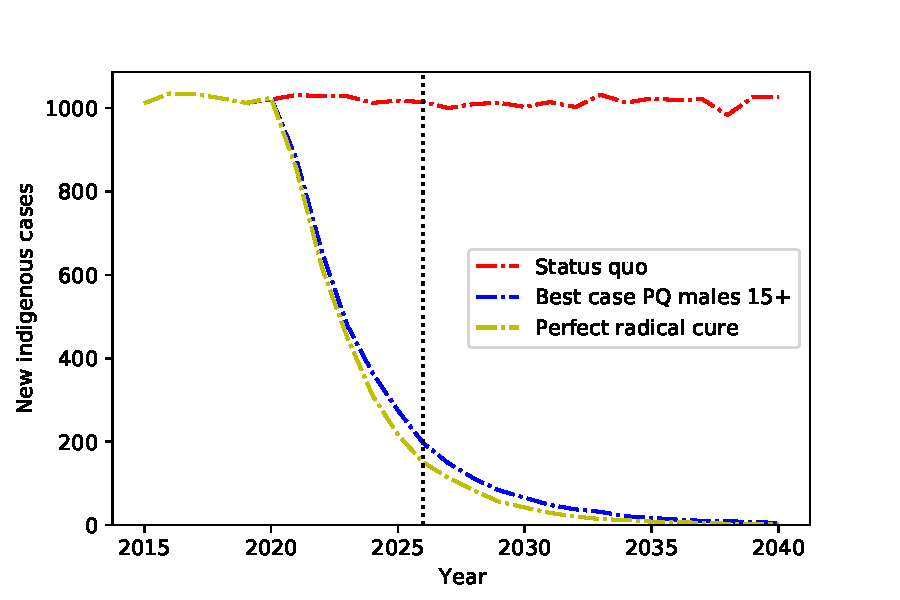
\includegraphics[width=.45\linewidth]{Battambang_high_indigenous_cases_Total.pdf}} 
\subcaptionbox{Total, high.\label{Battambang_high_active_cases_Total}}{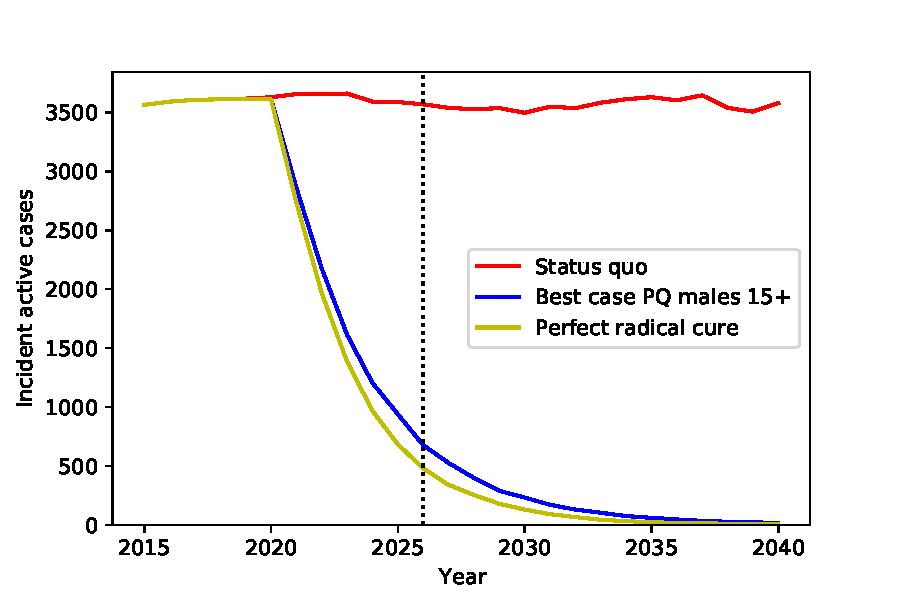
\includegraphics[width=.45\linewidth]{Battambang_high_active_cases_Total.pdf}} 
\subcaptionbox{Total, low.\label{Battambang_low_indigenous_cases_Total}}{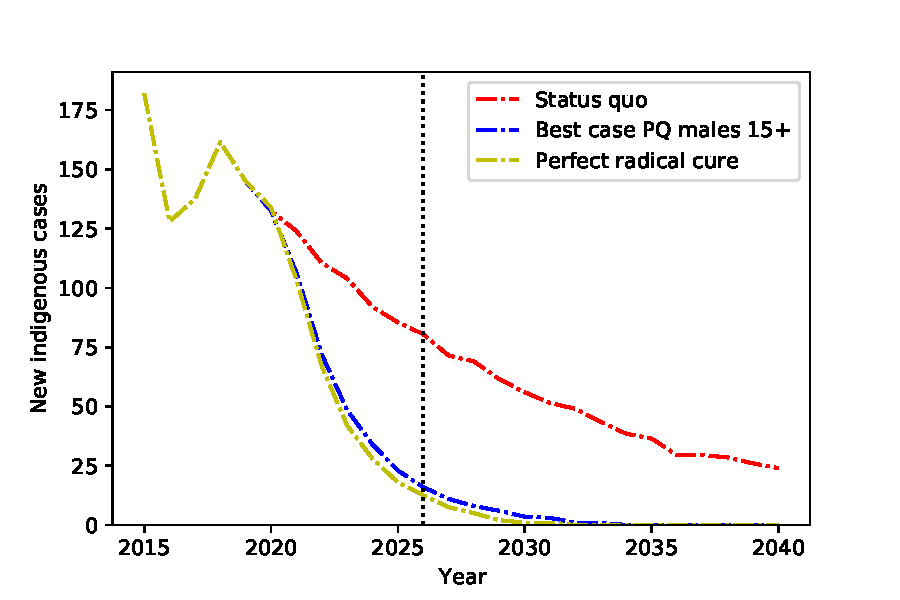
\includegraphics[width=.45\linewidth]{Battambang_low_indigenous_cases_Total.pdf}} 
\subcaptionbox{Total, low.\label{Battambang_low_active_cases_Total}}{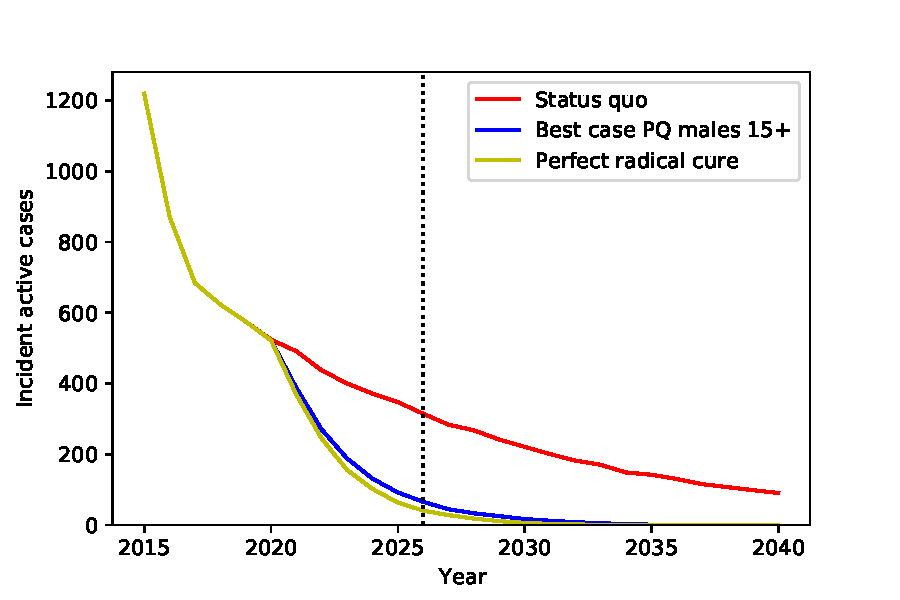
\includegraphics[width=.45\linewidth]{Battambang_low_active_cases_Total.pdf}} 
\caption{\csentence{\pq~intervention for \pv~in Battambang}. Lines represent annual medians for each individual year from 300 sampled model trajectories given the status quo and each radical cure scenario. Vertical dashed line is the December 2025 elimination target for \pv.}\label{fig:pq_Battambang}
\end{figure}

\begin{figure}[h!]
\centering
\subcaptionbox{Total, high.\label{Takeo_high_indigenous_cases_Total}}{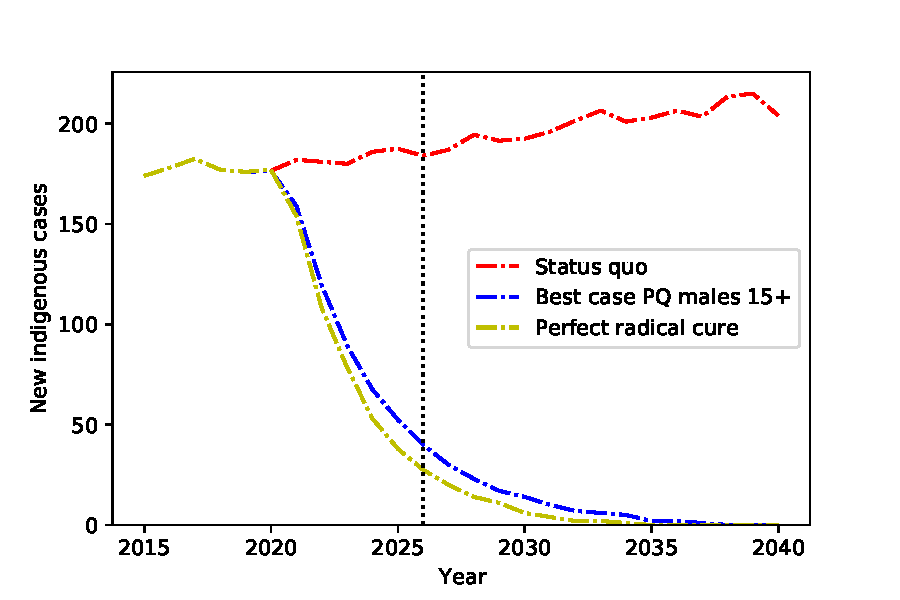
\includegraphics[width=.45\linewidth]{Takeo_high_indigenous_cases_Total.pdf}} 
\subcaptionbox{Total, high.\label{Takeo_high_active_cases_Total}}{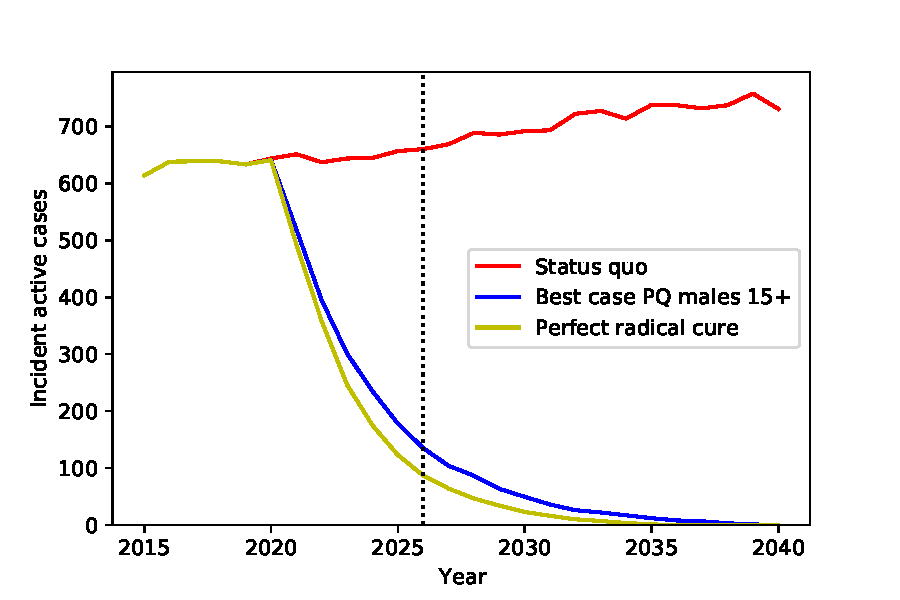
\includegraphics[width=.45\linewidth]{Takeo_high_active_cases_Total.pdf}} 
\subcaptionbox{Total, low.\label{Takeo_low_indigenous_cases_Total}}{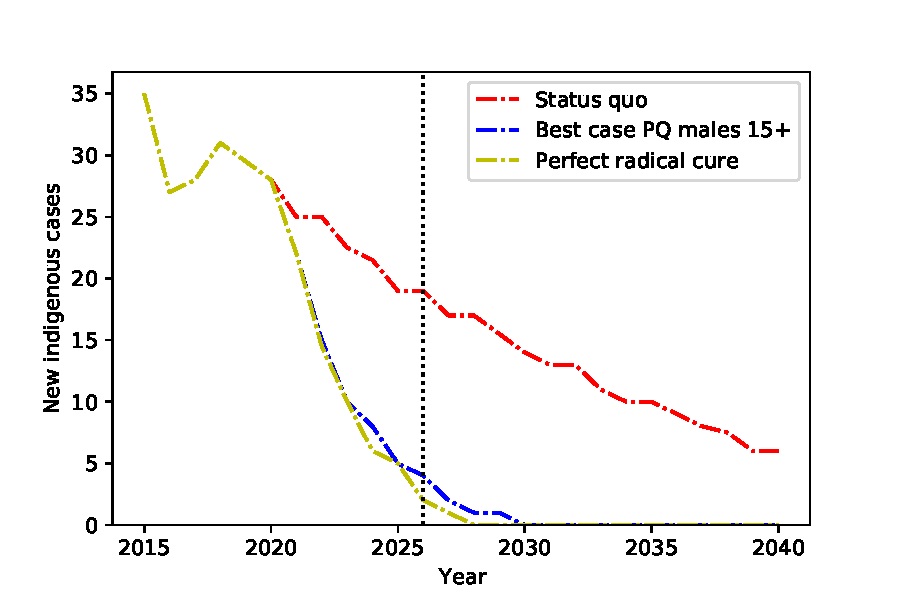
\includegraphics[width=.45\linewidth]{Takeo_low_indigenous_cases_Total.pdf}} 
\subcaptionbox{Total, low.\label{Takeo_low_active_cases_Total}}{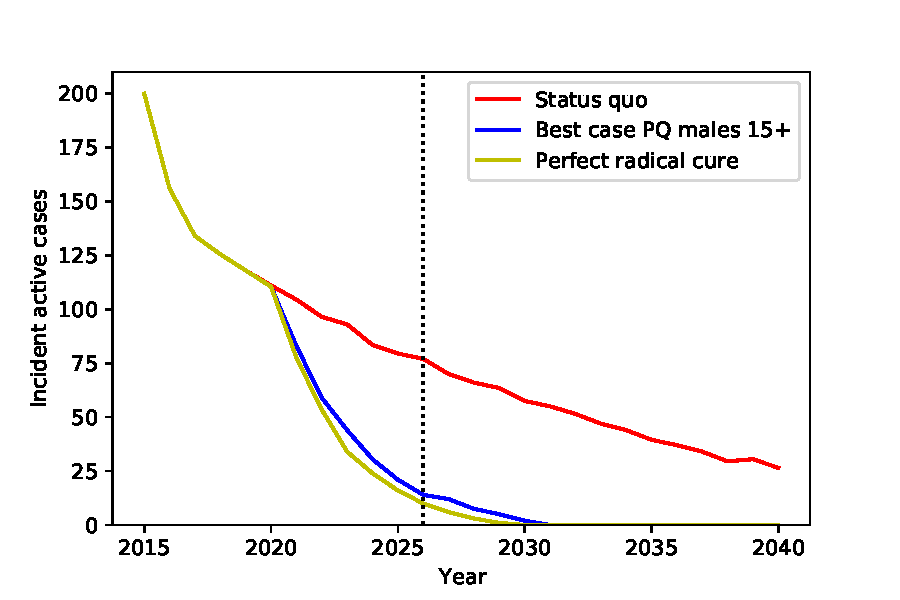
\includegraphics[width=.45\linewidth]{Takeo_low_active_cases_Total.pdf}} 
\caption{\csentence{\pq~intervention for \pv~in Takeo}. Lines represent annual medians for each individual year from 300 sampled model trajectories given the status quo and each radical cure scenario. Vertical dashed line is the December 2025 elimination target for \pv.}\label{fig:pq_Takeo}
\end{figure}

\begin{figure}[h!]
\centering
\subcaptionbox{Total, high.\label{Pailin_high_indigenous_cases_Total}}{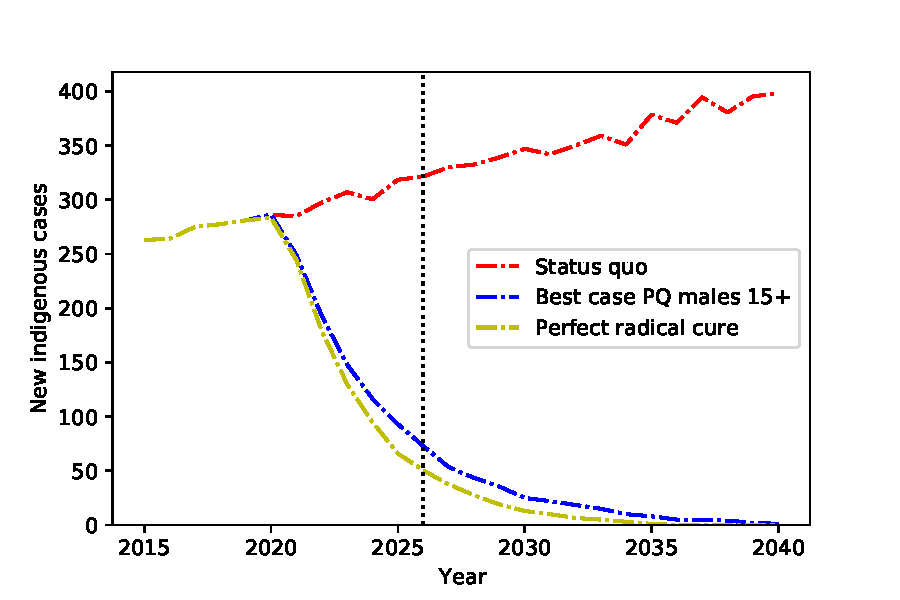
\includegraphics[width=.45\linewidth]{Pailin_high_indigenous_cases_Total.pdf}} 
\subcaptionbox{Total, high.\label{Pailin_high_active_cases_Total}}{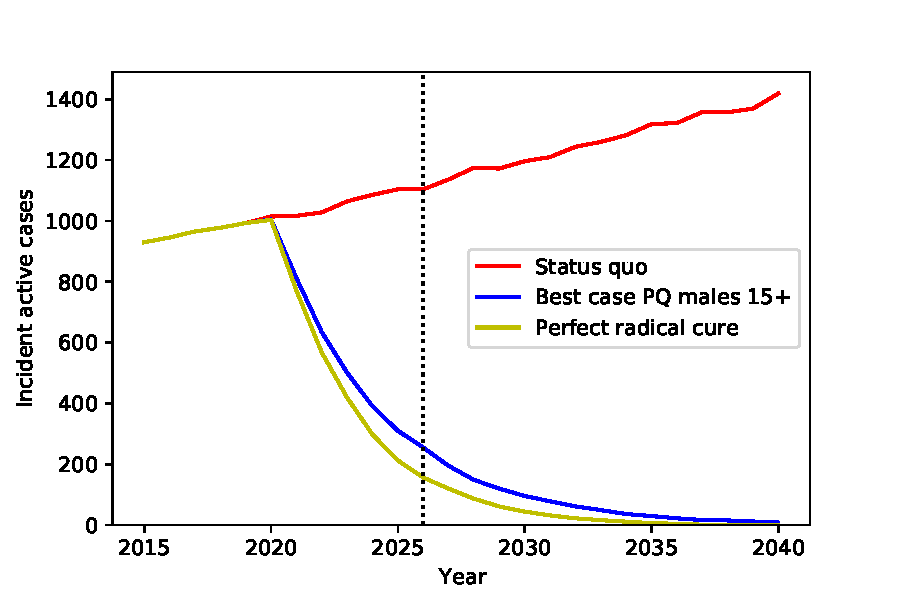
\includegraphics[width=.45\linewidth]{Pailin_high_active_cases_Total.pdf}} 
\subcaptionbox{Total, low.\label{Pailin_low_indigenous_cases_Total}}{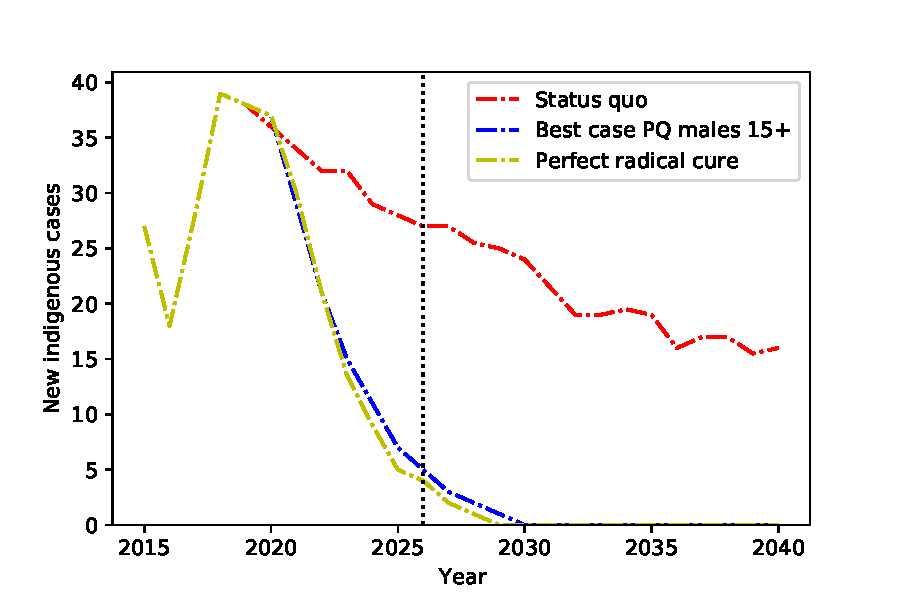
\includegraphics[width=.45\linewidth]{Pailin_low_indigenous_cases_Total.pdf}} 
\subcaptionbox{Total, low.\label{Pailin_low_active_cases_Total}}{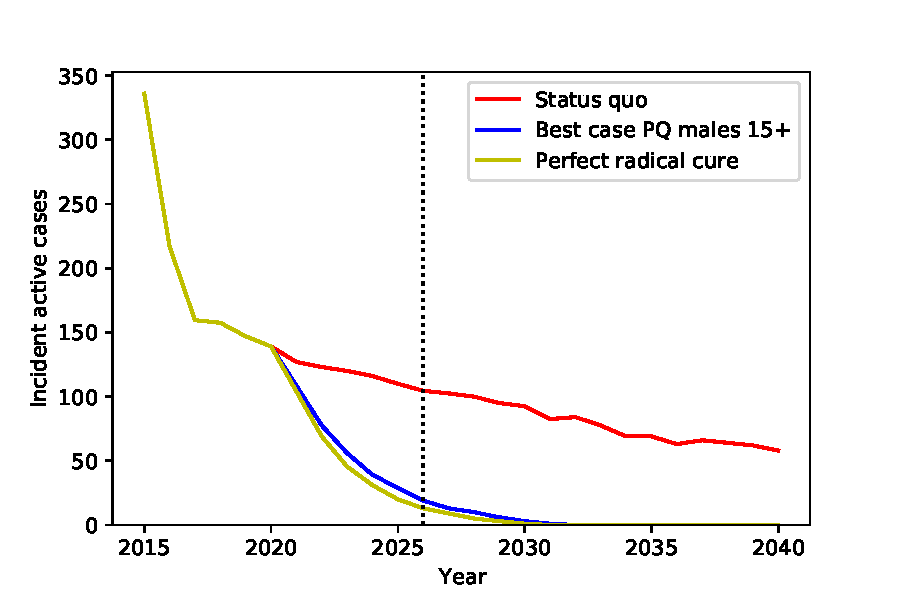
\includegraphics[width=.45\linewidth]{Pailin_low_active_cases_Total.pdf}} 
\caption{\csentence{\pq~intervention for \pv~in Pailin}. Lines represent annual medians for each individual year from 300 sampled model trajectories given the status quo and each radical cure scenario. Vertical dashed line is the December 2025 elimination target for \pv.}\label{fig:pq_Pailin}
\end{figure}

\end{backmatter}
\end{document}
